\chapter{Results}

About the final program results

There ar not just things to finish or implement, also, it is nedded to solve some actual problems. Most important of them are:

Signal Path glitch and page switching.................................

Less important, are: ......................................................

\begin{itemize}
	\item \textbf{Filter Algorithms:}
	
	\item \textbf{User Limitations:} For example, since we are using the Sounddevice library and managing both inputs as a single input stream, we have the limitation that both channels must come from the same sound card. However, the program currently allows the selection of different sound cards for each input channel.
	
\end{itemize}

\section{Final tests}

About testing program on real situations


\begin{figure}[H]
	\centering
	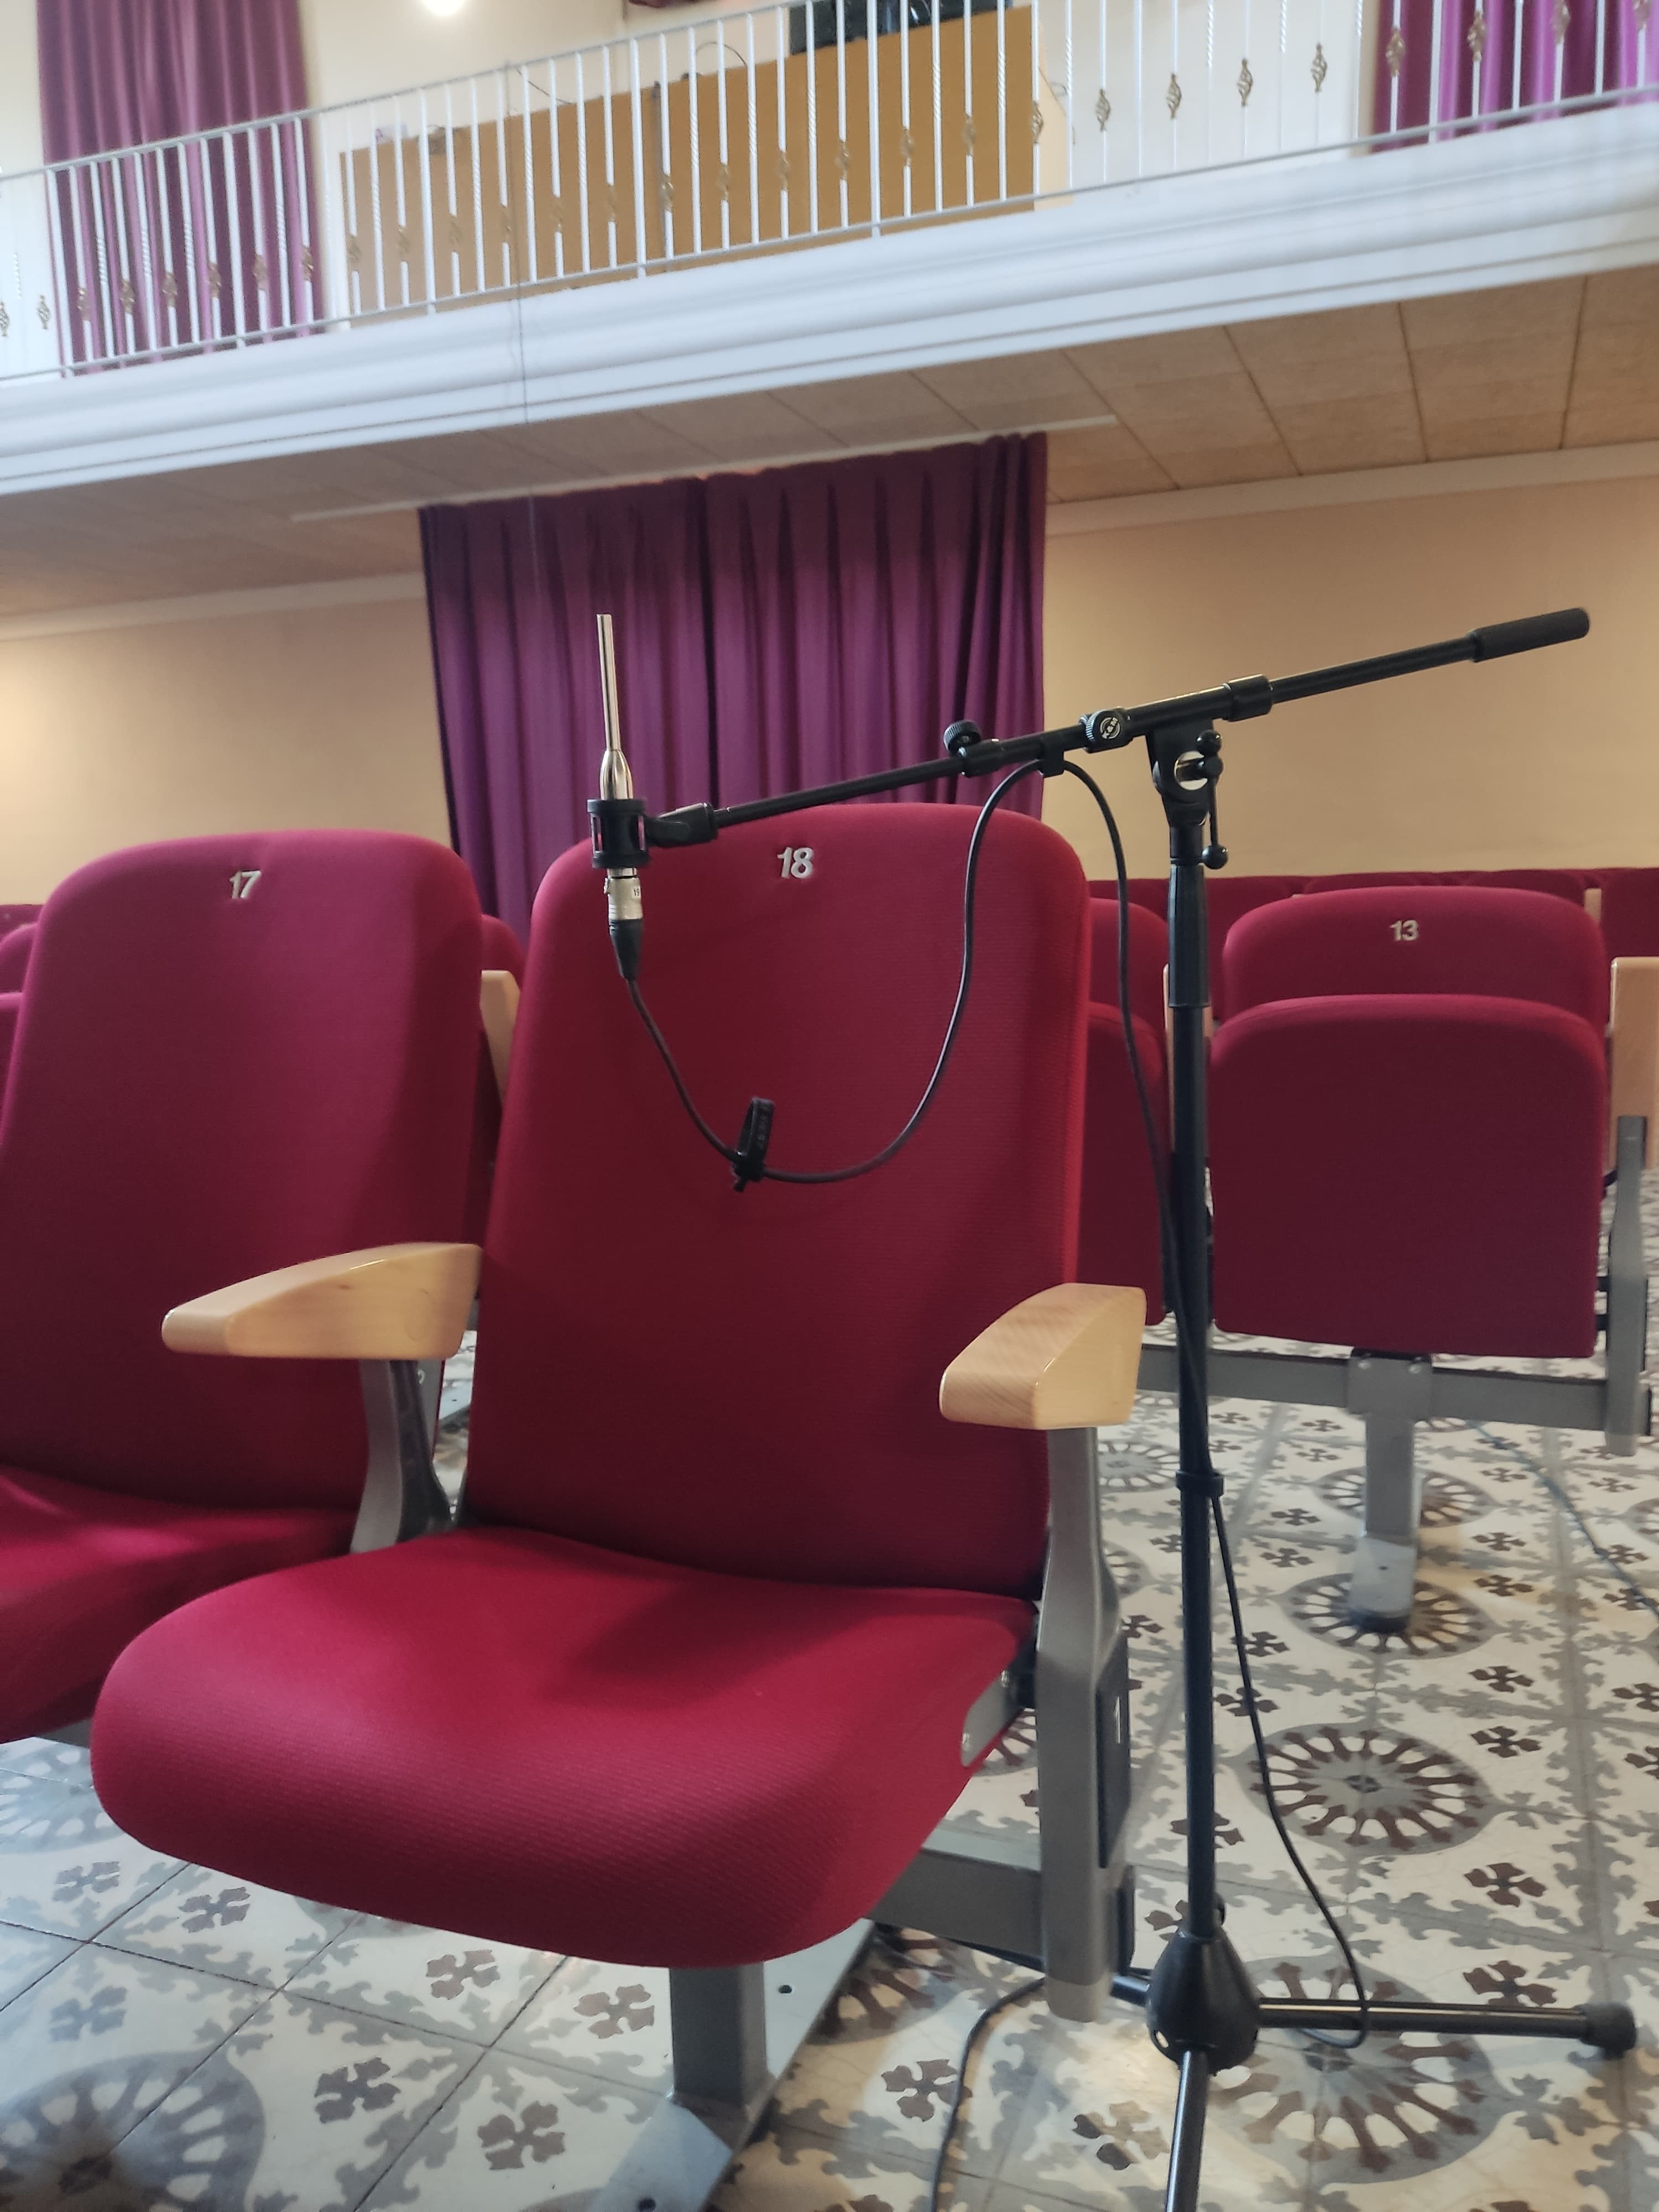
\includegraphics[width=0.6
	\linewidth]{Figures/Coro_micpos1.jpeg}
	\caption{Mic Height 1 .................................................}
	\label{fig:Mic_pos1}
\end{figure}

\begin{figure}[H]
	\centering
	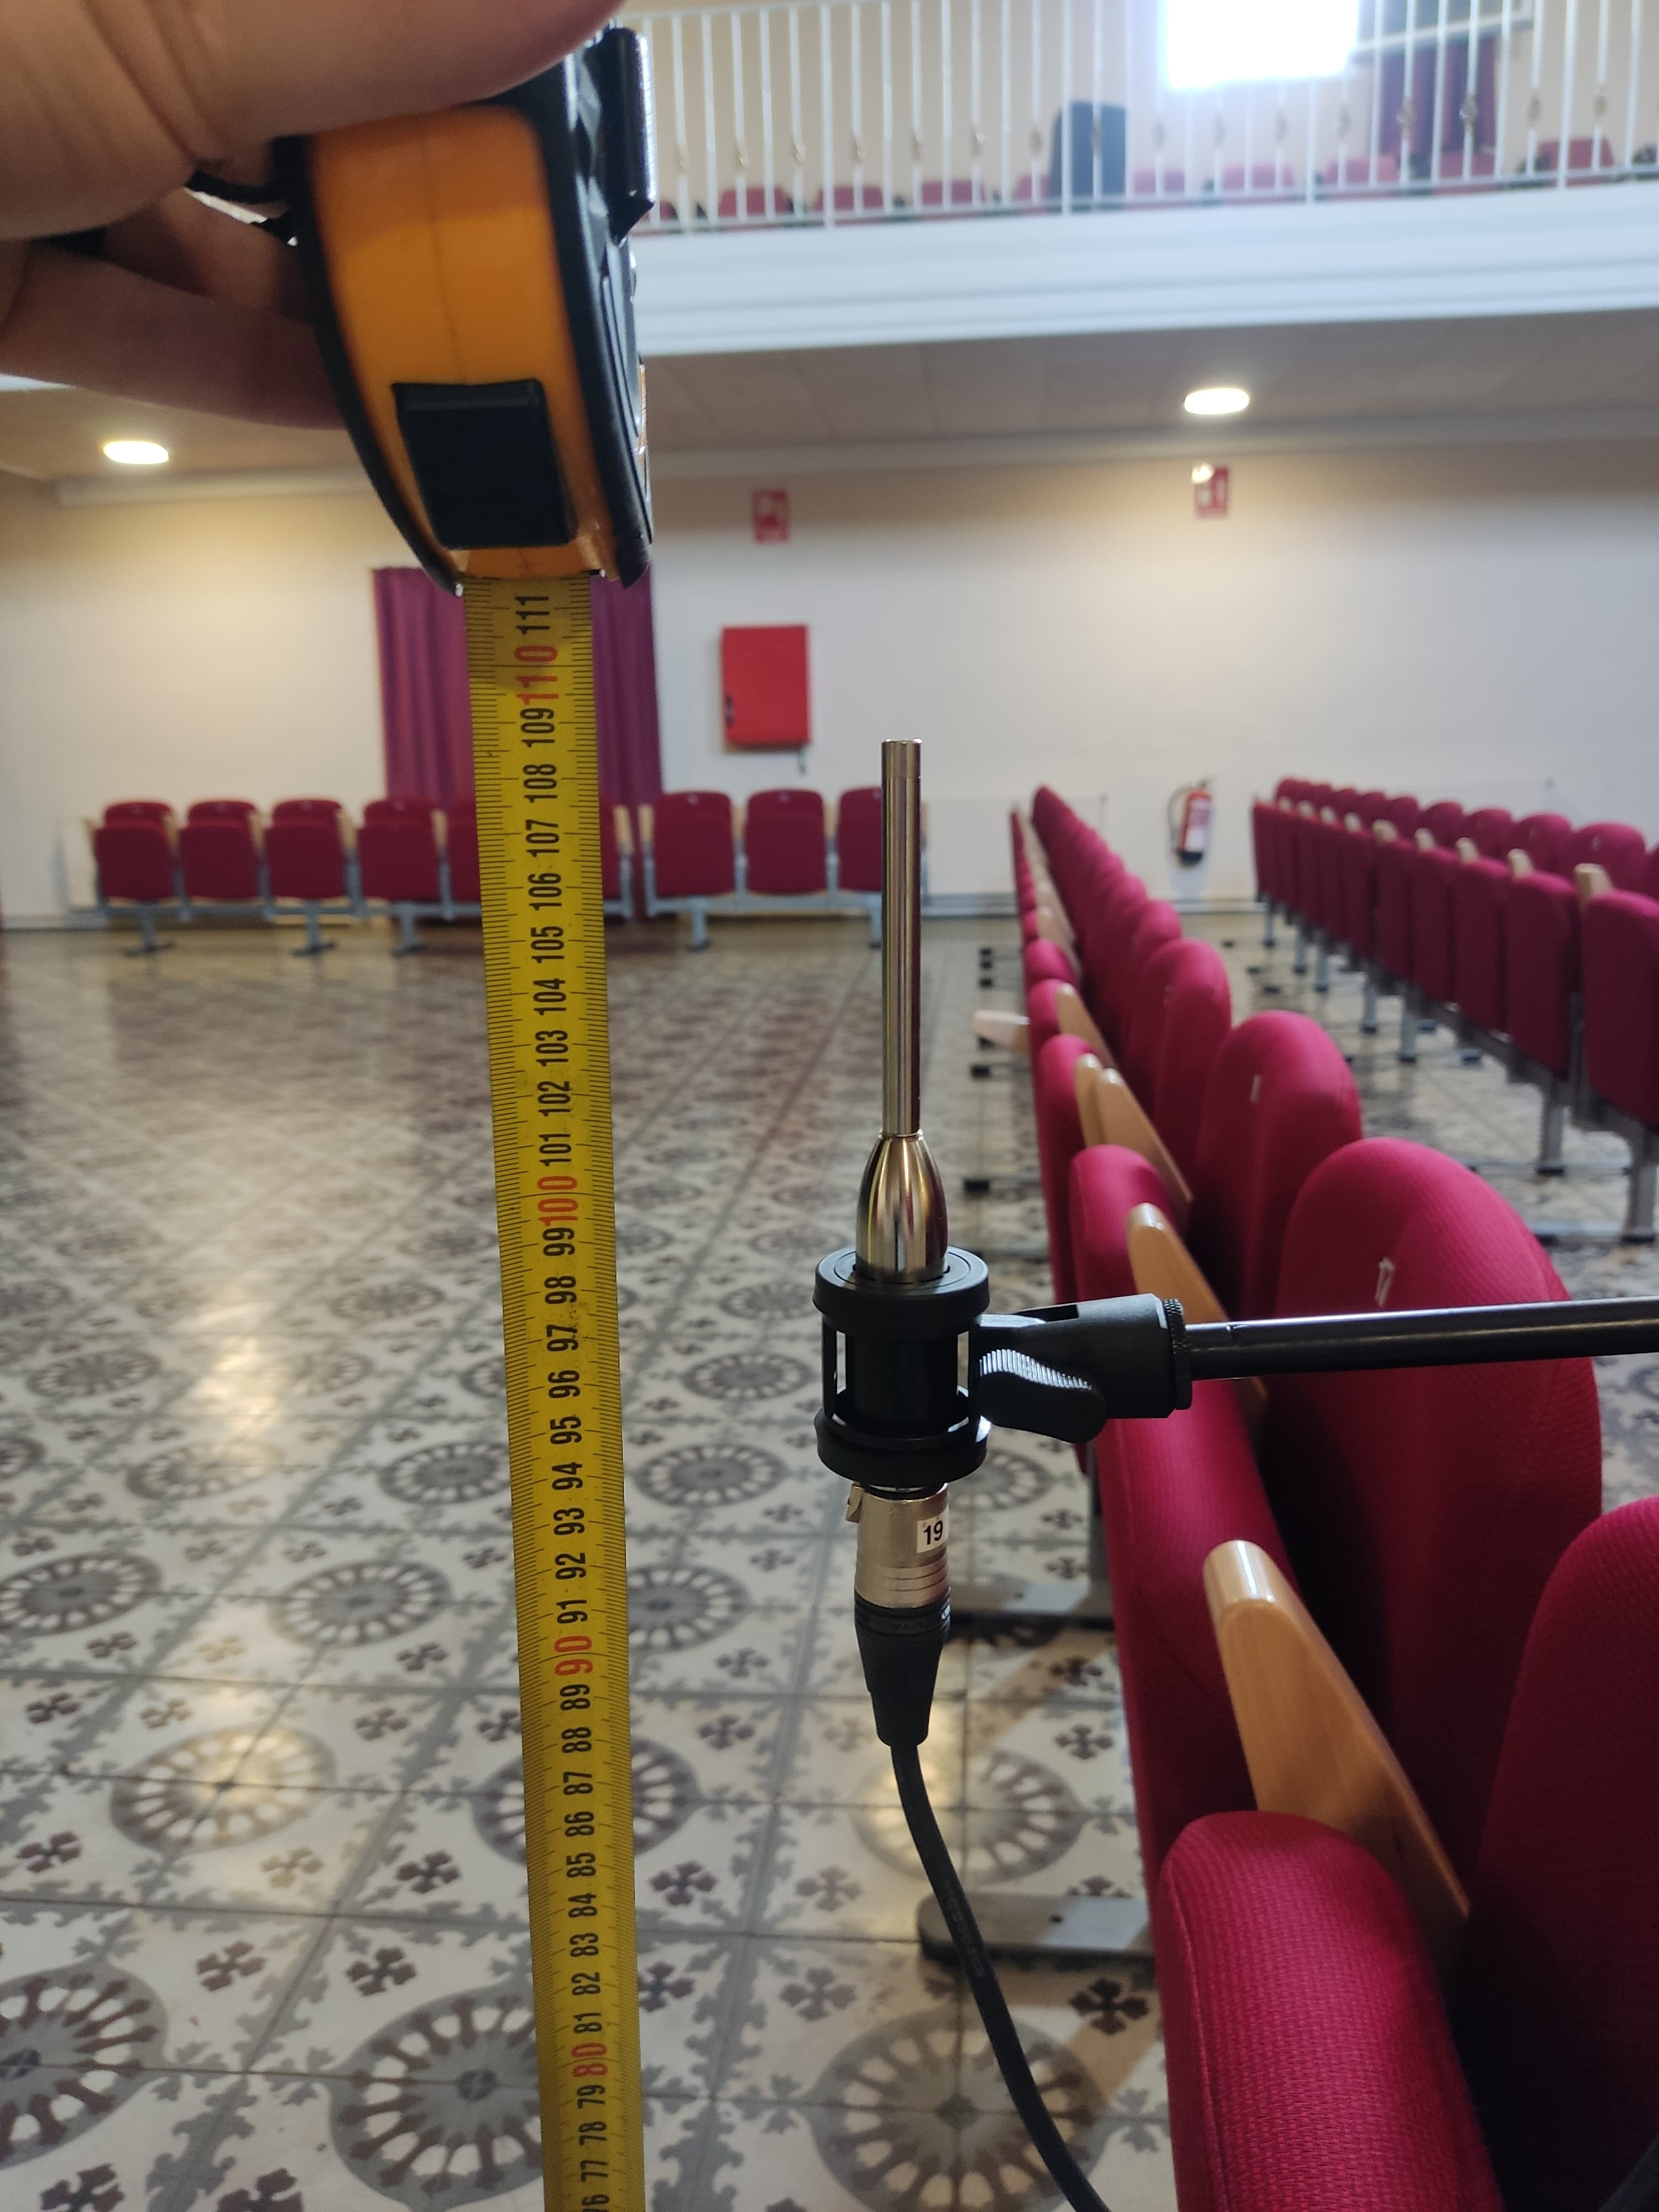
\includegraphics[width=0.6
	\linewidth]{Figures/Coro_micpos2.jpeg}
	\caption{Mic Height 2 .................................................}
	\label{fig:Mic_pos2}
\end{figure}

\begin{figure}[H]
	\centering
	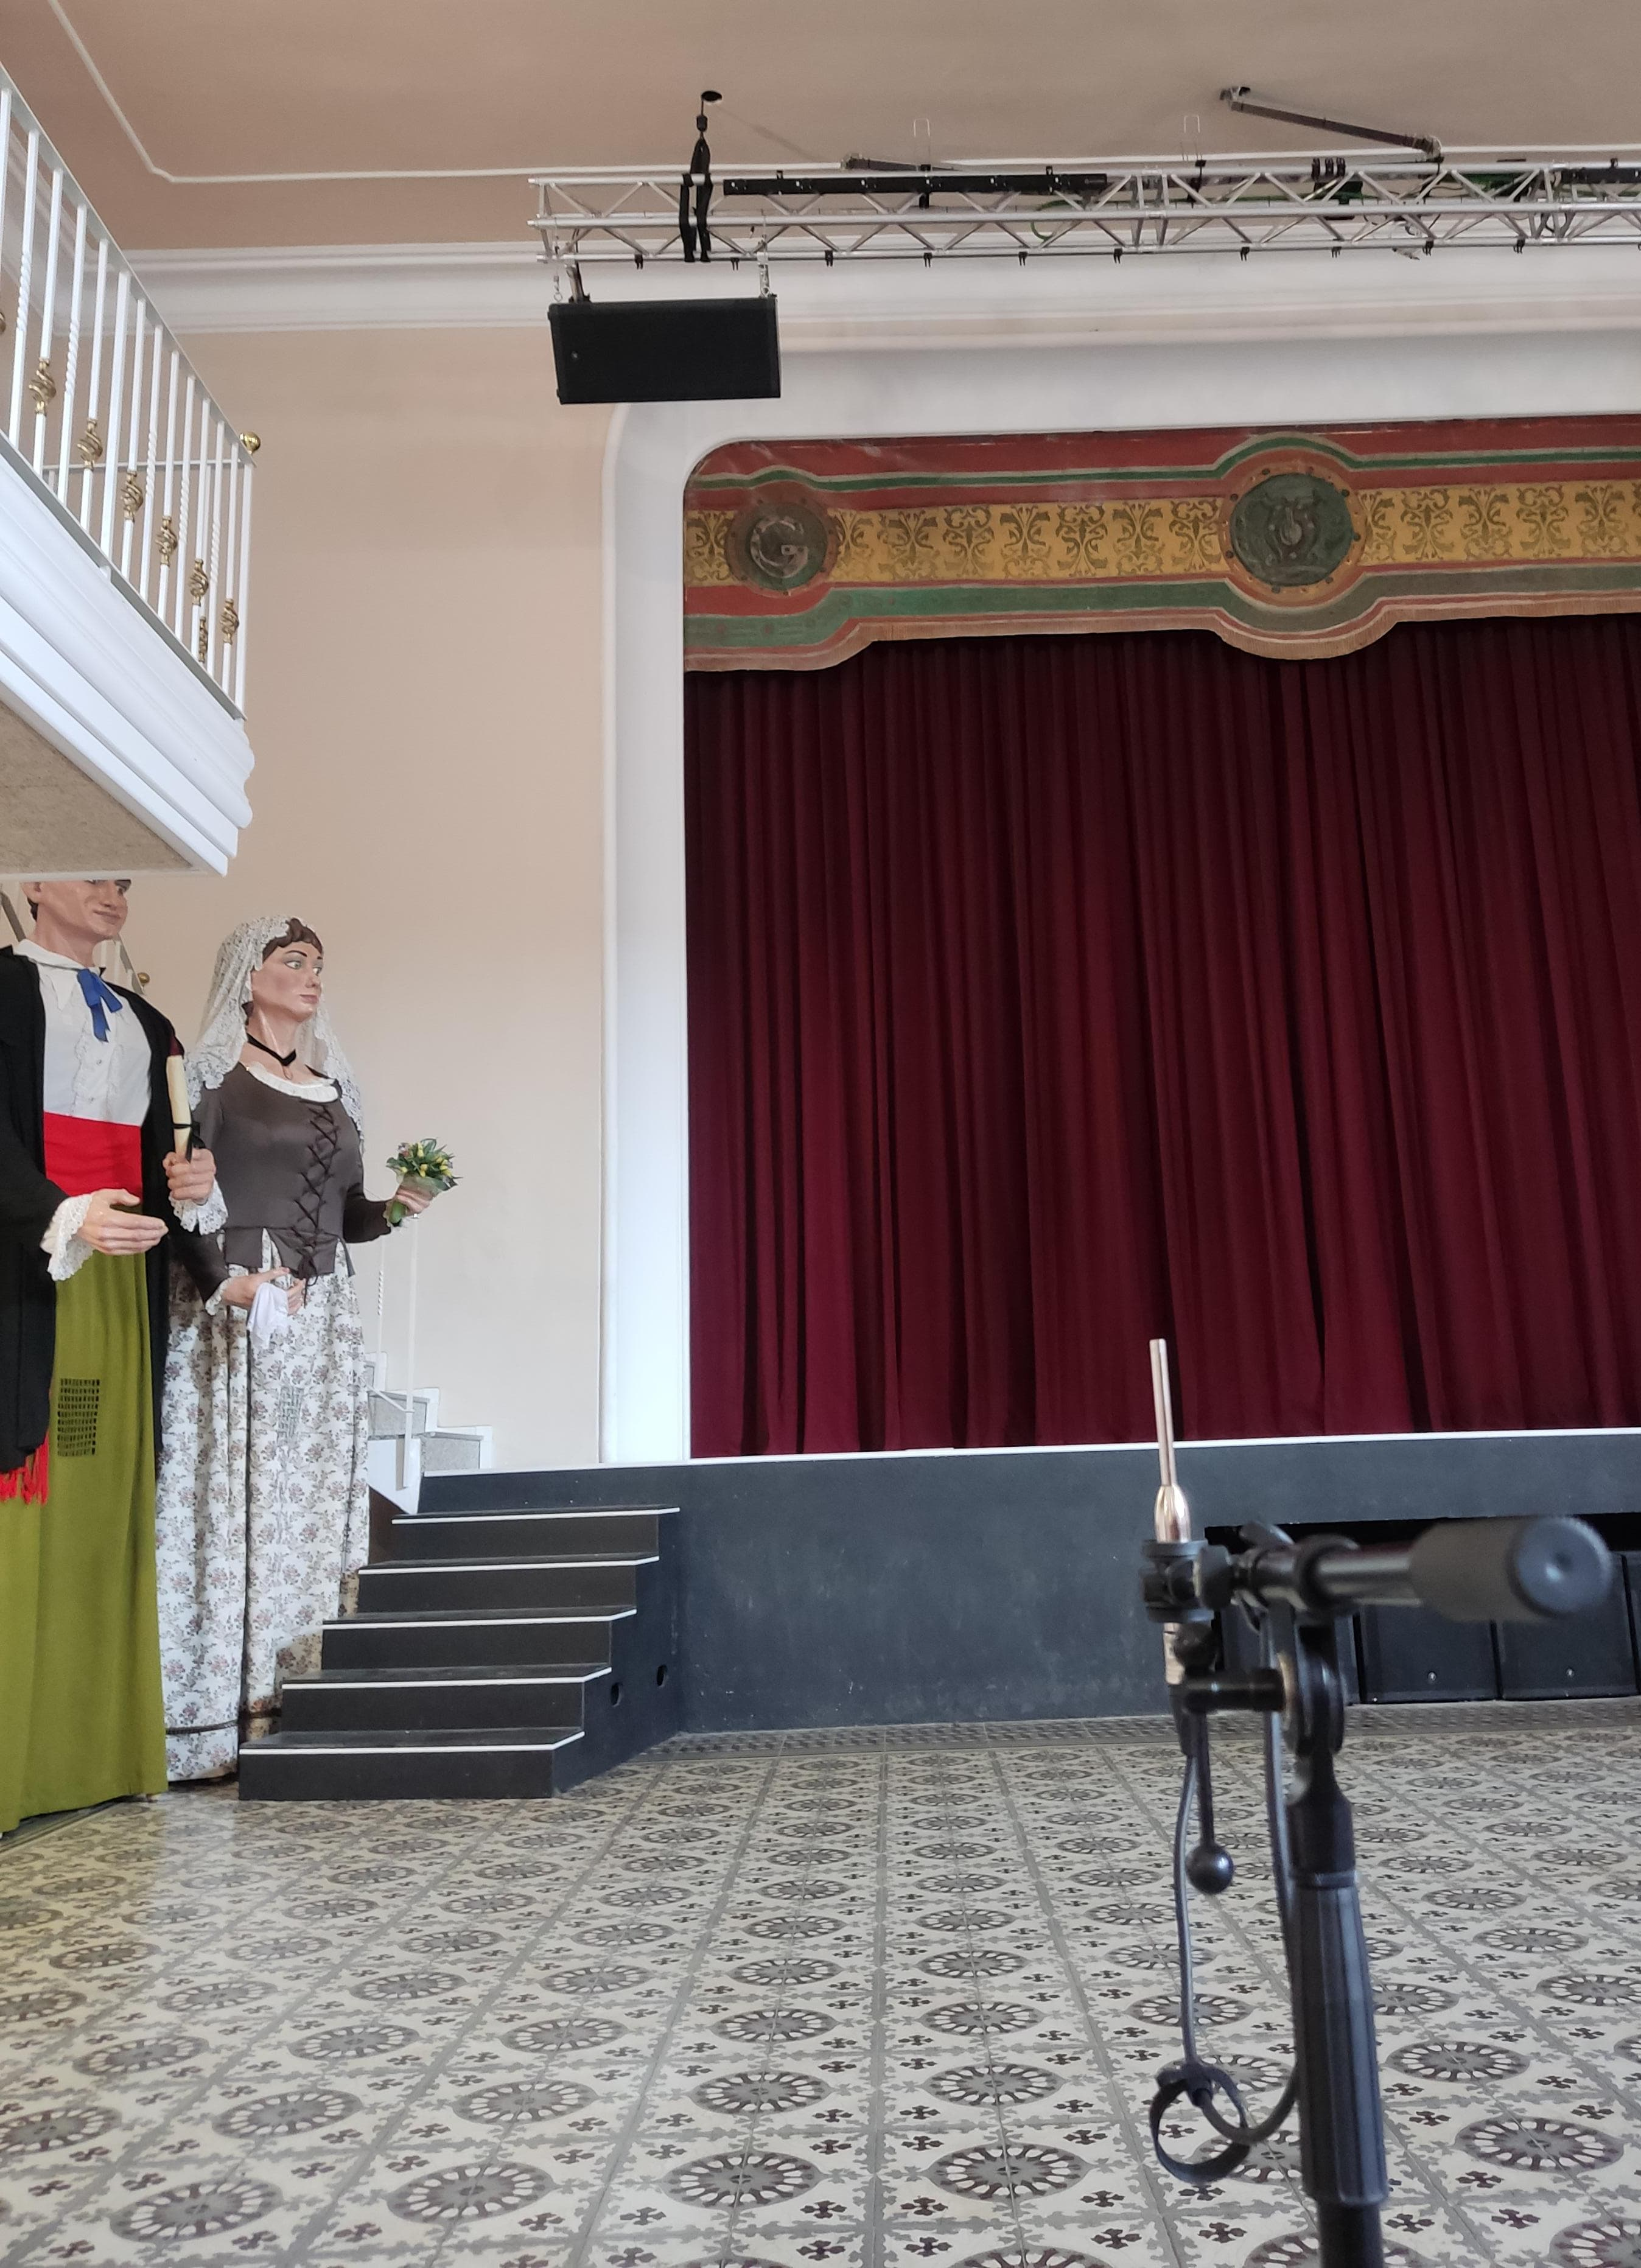
\includegraphics[width=0.6
	\linewidth]{Figures/Coro_micpos3.jpeg}
	\caption{Mic positioning .................................................}
	\label{fig:Mic_pos3}
\end{figure}

\begin{figure}[H]
	\centering
	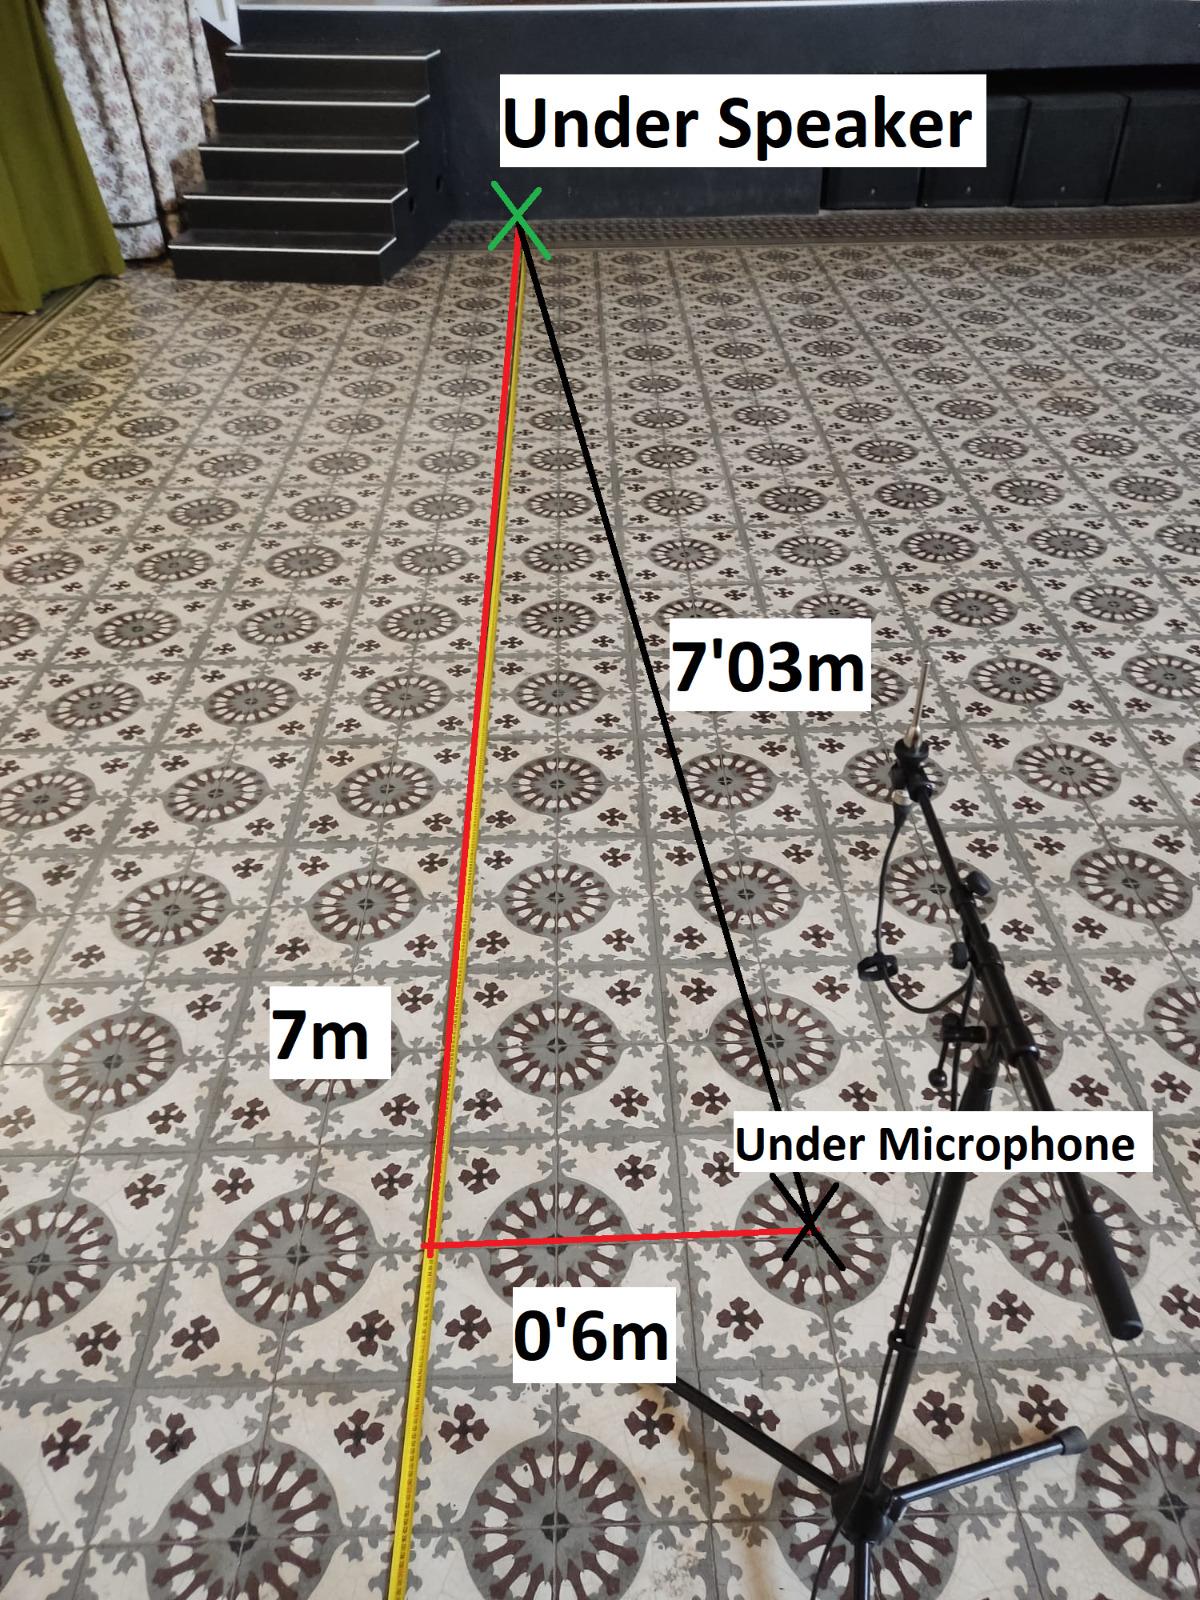
\includegraphics[width=0.6
	\linewidth]{Figures/Coro_floor_trigo.jpeg}
	\caption{Floor trigonometry of theater probes .................................................}
	\label{fig:Floor_section}
\end{figure}

\begin{figure}[H]
	\centering
	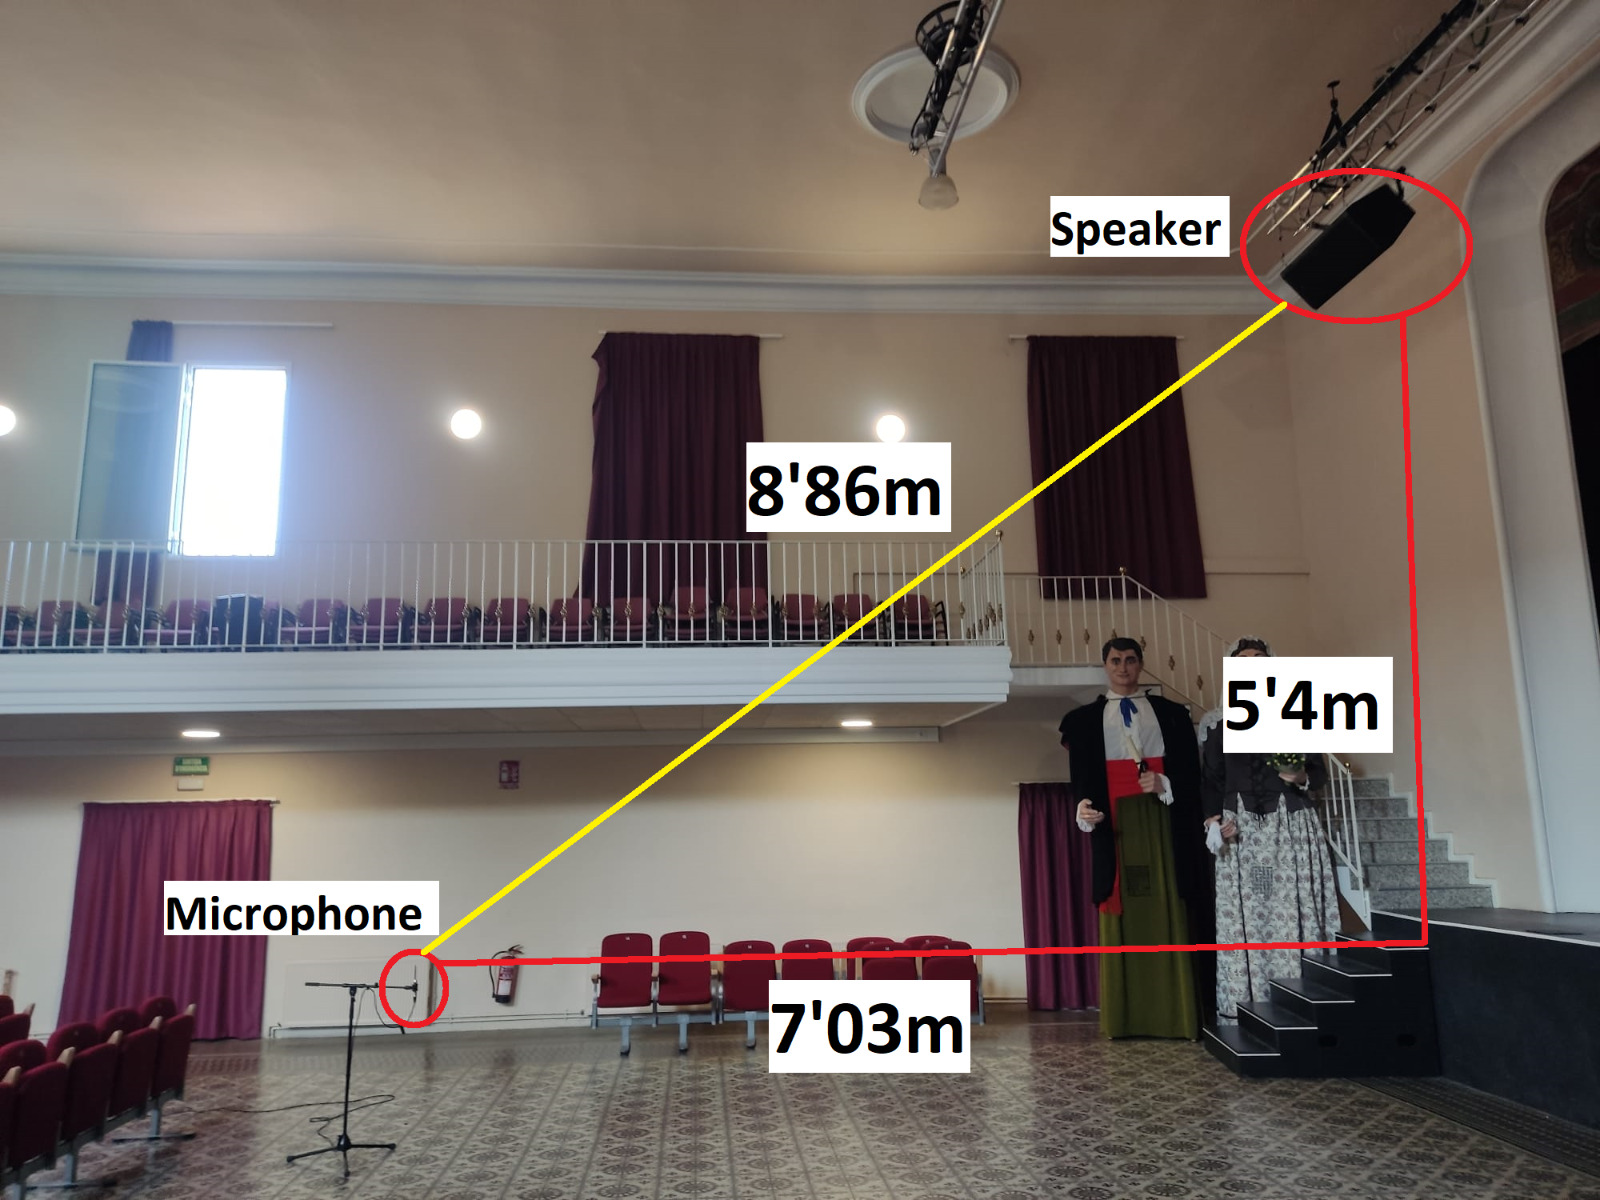
\includegraphics[width=1
	\linewidth]{Figures/Coro_section_trigo.jpeg}
	\caption{Distance calculation between Mic and Speak............................................}
	\label{fig:asdf}
\end{figure}

Speaker at 6.5m height, restar 1.1m from height of microphone ......................................

\begin{figure}[H]
	\centering
	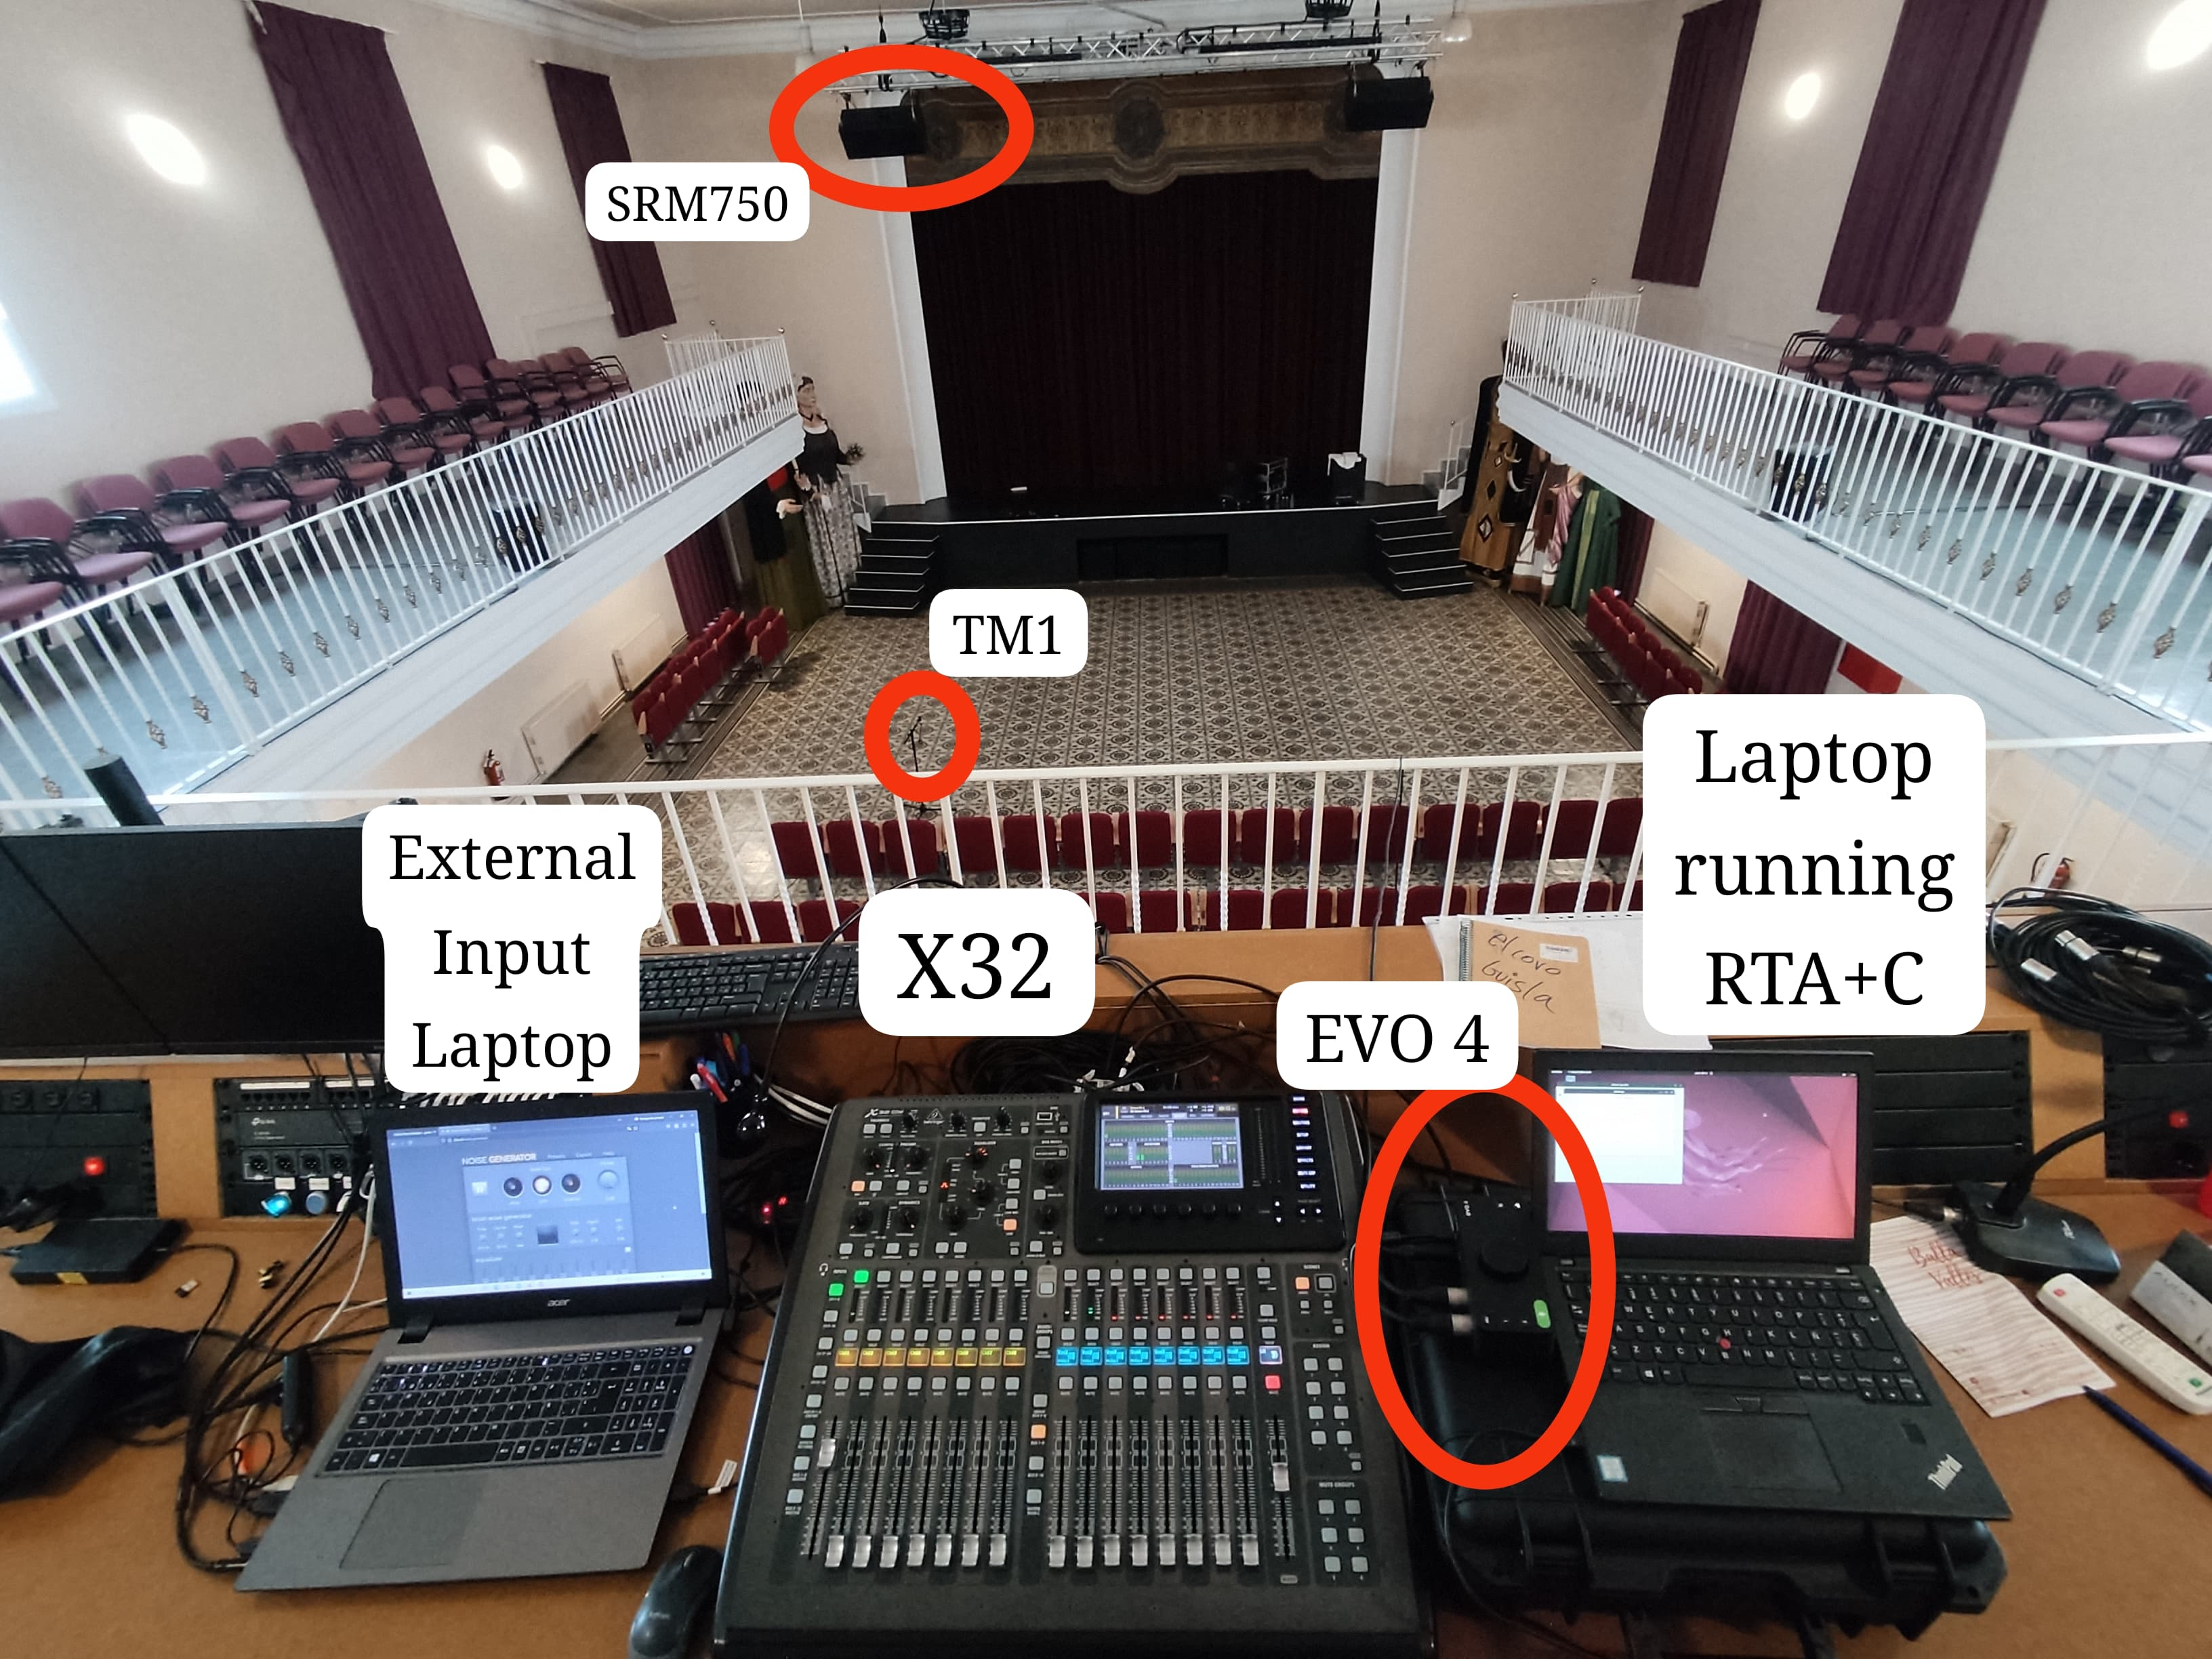
\includegraphics[width=1
	\linewidth]{Figures/Coro_setup.jpeg}
	\caption{Theater test setup .................................................}
	\label{fig:Coro_setup}
\end{figure}

EVO 4 is our soundcard..........................................................

Conection SETUP --> In order to compare our software solution with other tools, Have to connect to split all signals to both devices (Also needed to send the output signal to speaker)......................................................................................................

\begin{figure}[H]
	\begin{center}
		\vspace{-2mm}
		\tikzsetnextfilename{connectio_setup}
		\begin{tikzpicture}[node distance=30mm,on grid,auto, scale=1, bend angle=45]
			
			every node/.style={font=\small};
			
			\node (q_ext) [draw, rectangle, minimum size=1cm] {Laptop (source of sound)};
			\node (q_X32_ext) [draw, rectangle, minimum size=1cm, right=of q_ext, xshift=2cm]{X32 - External Input};
			\node (q_evo_ext) [draw, rectangle, minimum size=1cm, right=of q_X32_ext, xshift=2cm]{EVO 4 External Input};
			\node (q_evo_out) [draw, rectangle, minimum size=1cm, below=of q_evo_ext]{EVO 4 Output to System};
			\node (q_X32_out) [draw, rectangle, minimum size=1cm, below=of q_X32_ext]{X32 - Output to System};
			\node (q_spk) [draw, rectangle, minimum size=1cm, below=of q_ext]{Speaker};
			\node (q_mic) [draw, rectangle, minimum size=1cm, below=of q_spk]{Microphone};
			\node (q_X32_in) [draw, rectangle, minimum size=1cm, below=of q_X32_out]{X32 - Input from System};
			\node (q_evo_in) [draw, rectangle, minimum size=1cm, below=of q_evo_out]{EVO 4 Input from System};
			
			\draw[blue, very thick, ->] (q_ext) edge node {} (q_X32_ext);
			\draw[blue, very thick, ->] (q_X32_ext) edge node {} (q_evo_ext);
			\draw[blue, very thick, ->] (q_evo_out) edge node {} (q_X32_out);
			\draw[blue, very thick, ->] (q_X32_out) edge node {} (q_spk);
			\draw[red, very thick, ->] (q_spk) edge [bend left=30] node {System} (q_mic);
			\draw[blue, very thick, ->] (q_mic) edge node {} (q_X32_in);
			\draw[blue, very thick, ->] (q_X32_in) edge node {} (q_evo_in);
			\draw[green, dotted, very thick, ->] (q_X32_ext) edge [bend right=30] node {Bypass or EQ using X32} (q_X32_out);
			\draw[blue,, dotted, very thick, ->] (q_evo_ext) edge [bend right=30] node {Bypass or EQ using RTA+C} (q_evo_out);
			%\draw[blue, very thick, ->] (q_out_bf) edge node {} (q_out_st);
			%\draw[blue, very thick, ->] (q_out_st) edge node {} (q_out);
			
			
		\end{tikzpicture}
		\vspace{-2mm}
	\end{center}
	\caption{Conection Setup ....................................}
\end{figure}

To compare between X32 and RTA+C, I was switching between two inputs that have conceptuall stage of X32 - Output to System from last schematic.........................................


\begin{figure}[H]
	\centering
	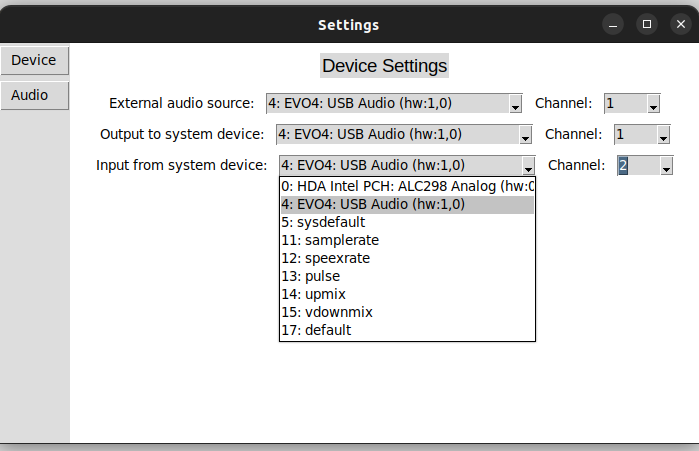
\includegraphics[width=0.6
	\linewidth]{Figures/Coro_Device_settings.png}
	\caption{Device Settings........................................................................}
	\label{fig:Coro_device_settings}
\end{figure}

Left default audio settings ............................................................

\begin{figure}[H]
	\centering
	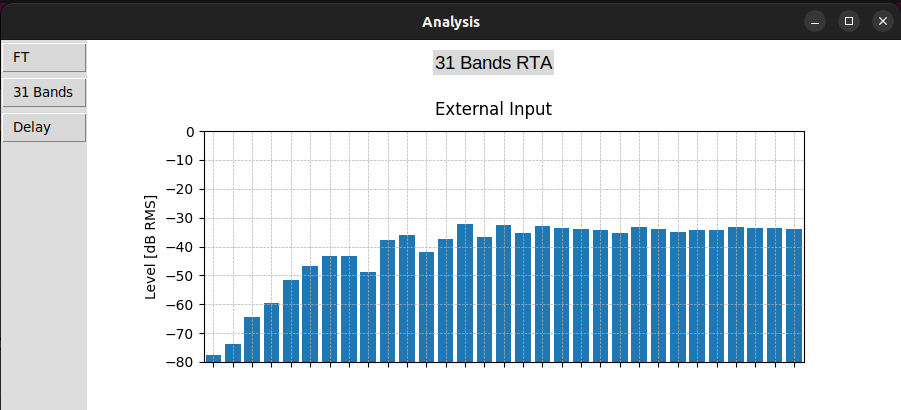
\includegraphics[width=0.6
	\linewidth]{Figures/Coro_Pink_Bad.png}
	\caption{Second delay measurement..............................................................}
	\label{fig:Coro_Bad_Pink}
\end{figure}

\begin{figure}[H]
	\centering
	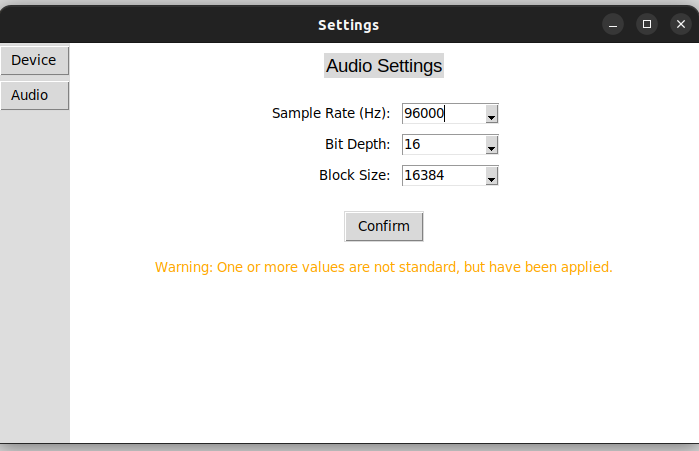
\includegraphics[width=0.6
	\linewidth]{Figures/Coro_audio_settings.png}
	\caption{Audio Settings........................................................................}
	\label{fig:Coro_audio_settings}
\end{figure}

Bloc Size too small --> Change BlockSize to 16384 --> 96KHz = 170.7ms ...........................................

\begin{figure}[H]
	\centering
	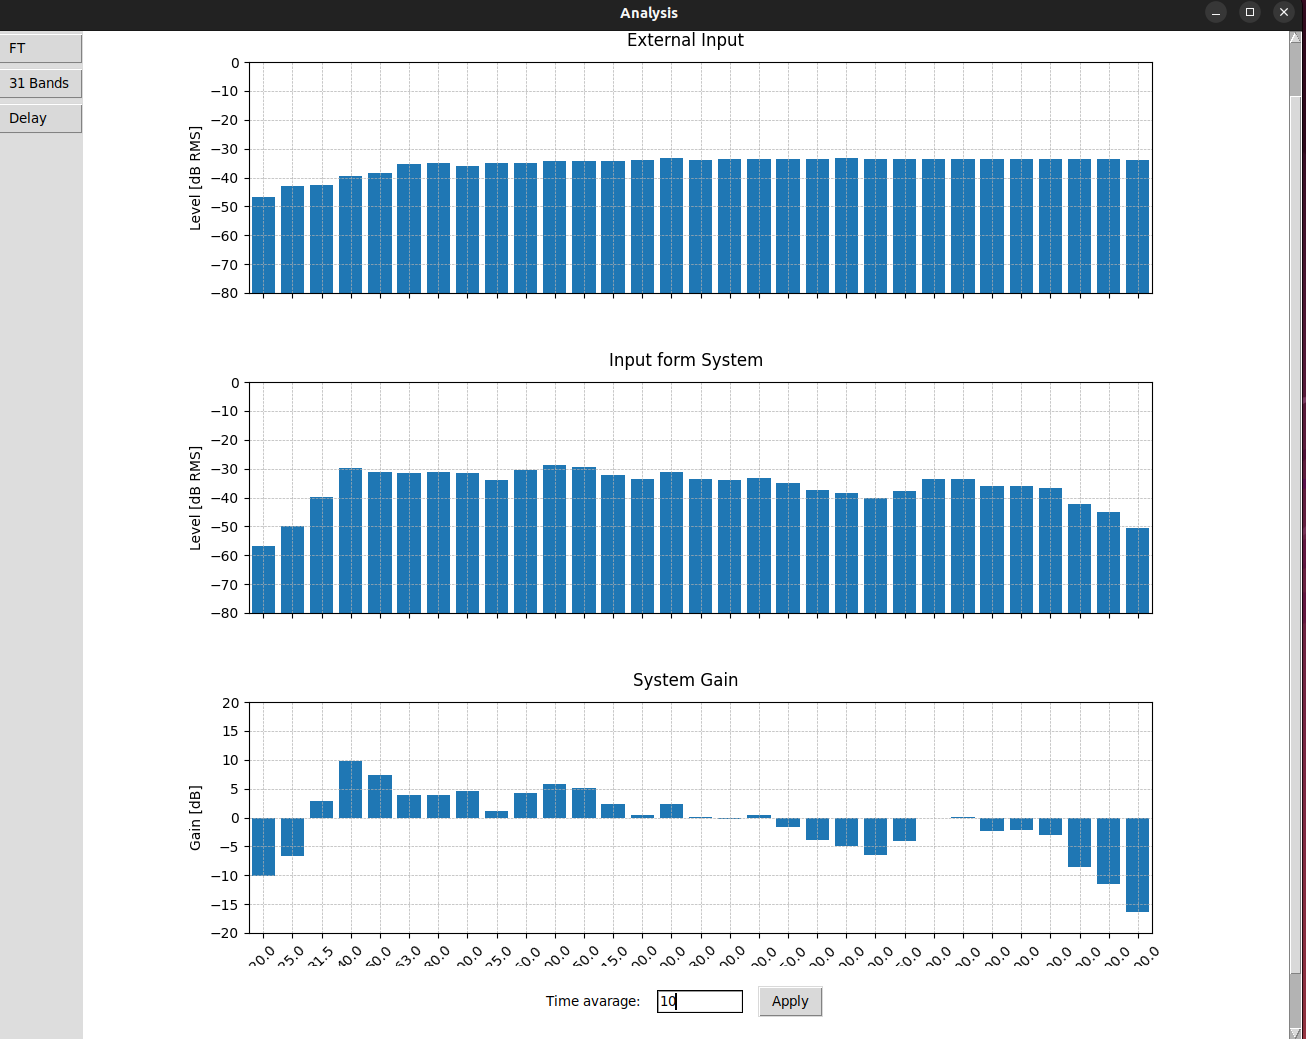
\includegraphics[width=0.6
	\linewidth]{Figures/Coro_Pink_Good.png}
	\caption{Second delay measurement..............................................................}
	\label{fig:Coro_Good_Pink}
\end{figure}

\begin{figure}[H]
	\centering
	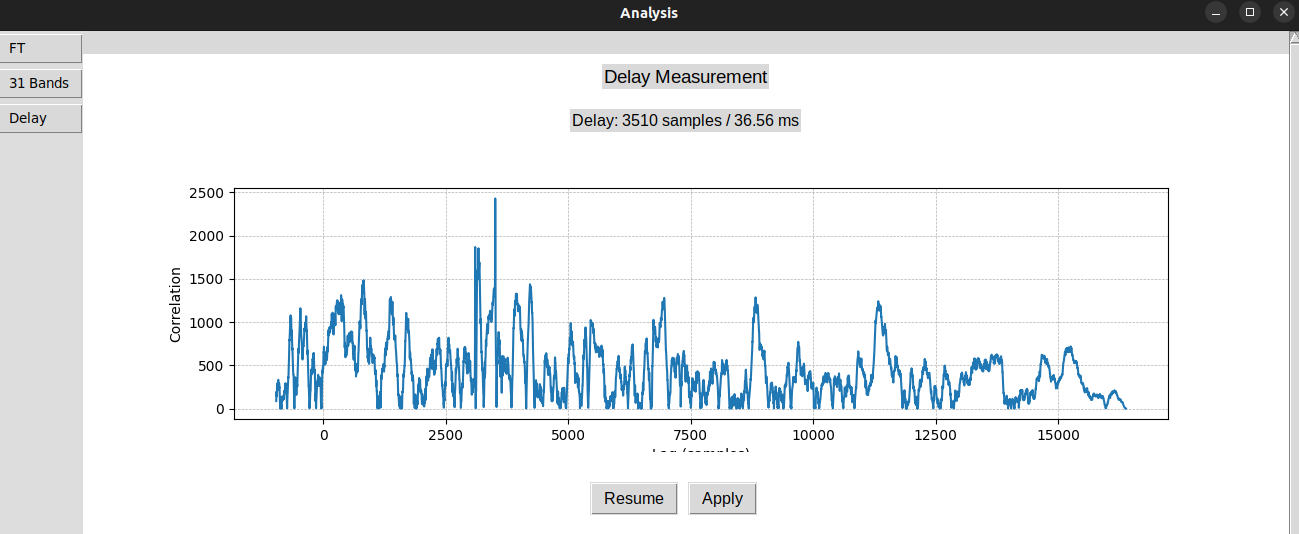
\includegraphics[width=0.6
	\linewidth]{Figures/Coro_Delay.png}
	\caption{First delay measurement...............................................................}
	\label{fig:Coro_delay1}
\end{figure}

36.56ms = 12.43m (340m/s) .........................................................................

\begin{figure}[H]
	\centering
	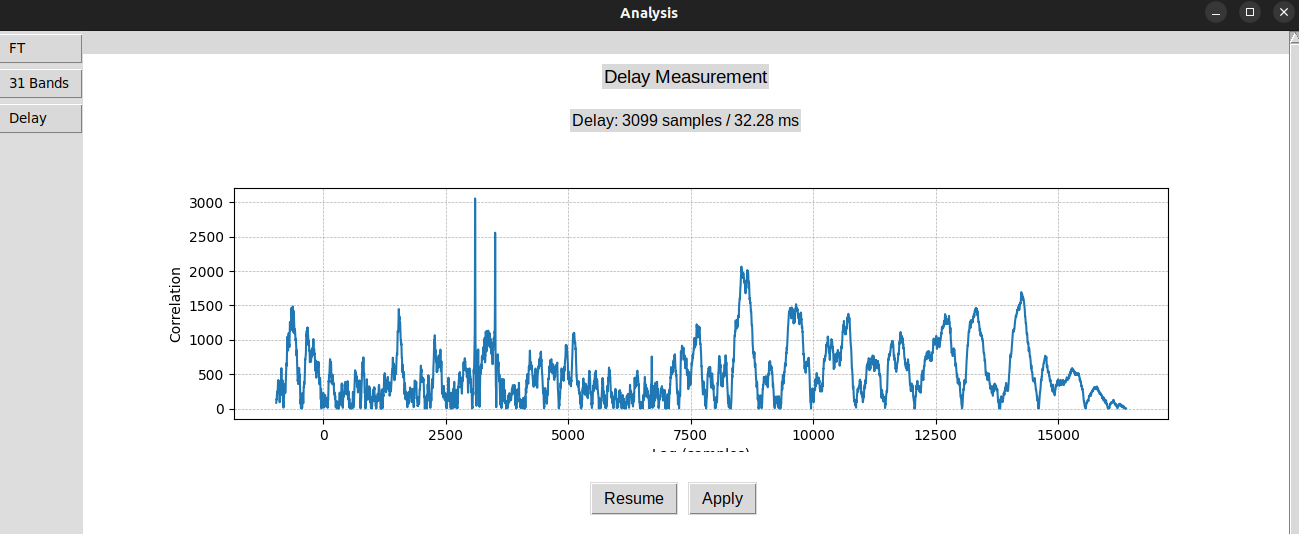
\includegraphics[width=0.6
	\linewidth]{Figures/Coro_delay_2.png}
	\caption{Second delay measurement..............................................................}
	\label{fig:Coro_delay2}
\end{figure}

32.28ms = 10.98m (340m/s) ..............................................................

\begin{figure}[H]
	\centering
	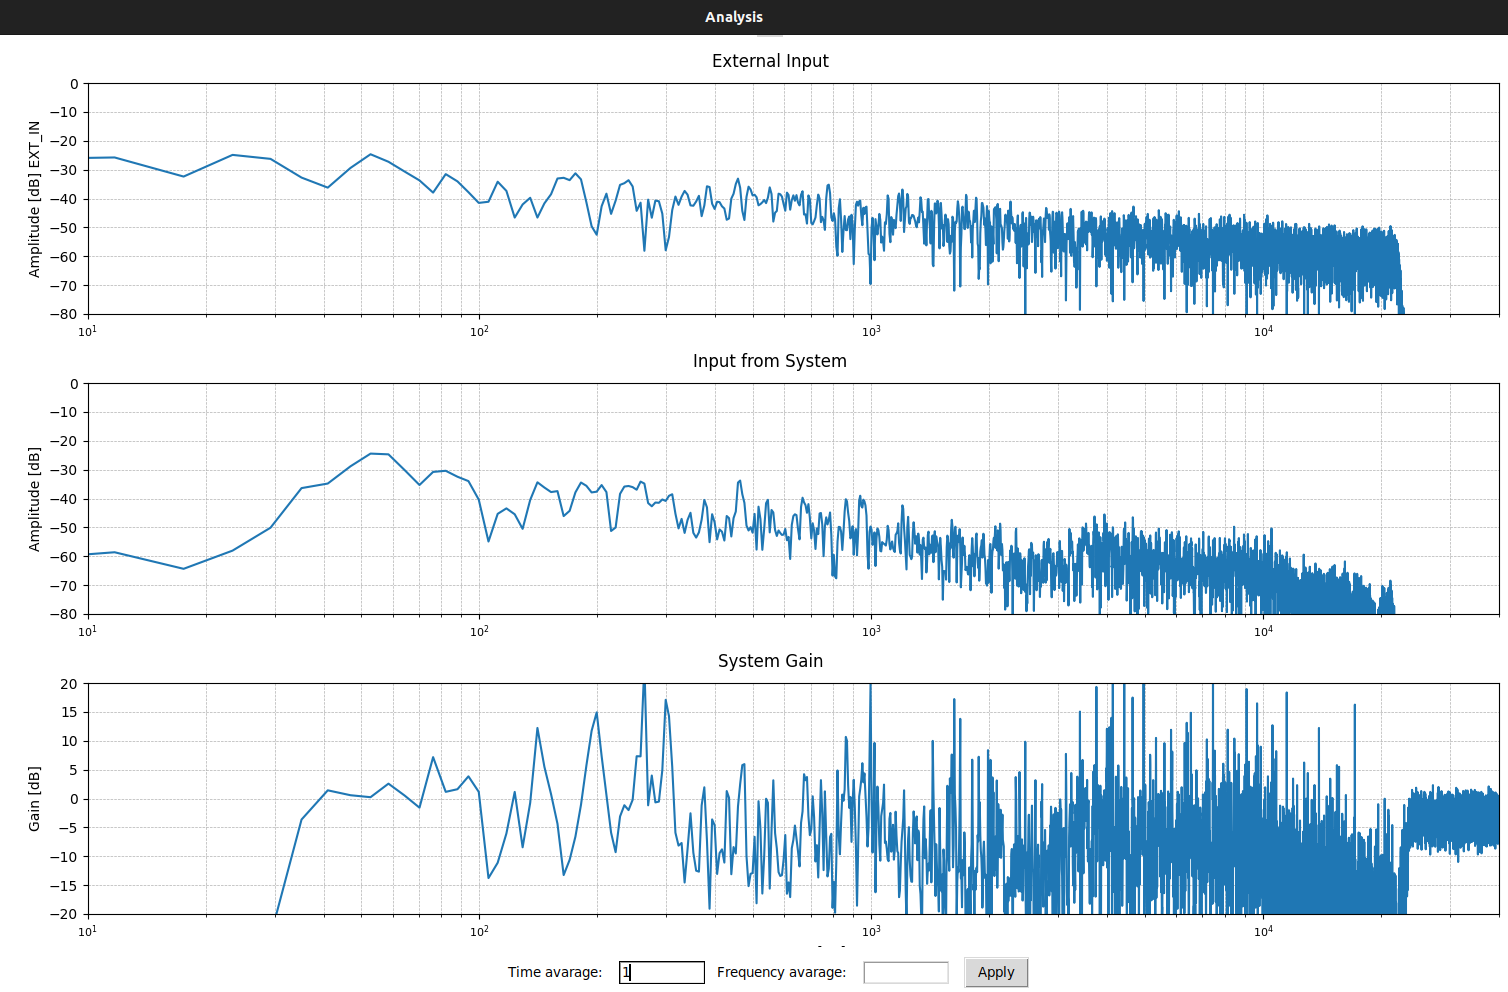
\includegraphics[width=0.6
	\linewidth]{Figures/Coro_FT_NO_av.png}
	\caption{FT - Pink Noise - No Avarage..............................................................}
	\label{fig:Coro_FT_no_av}
\end{figure}

\begin{figure}[H]
	\centering
	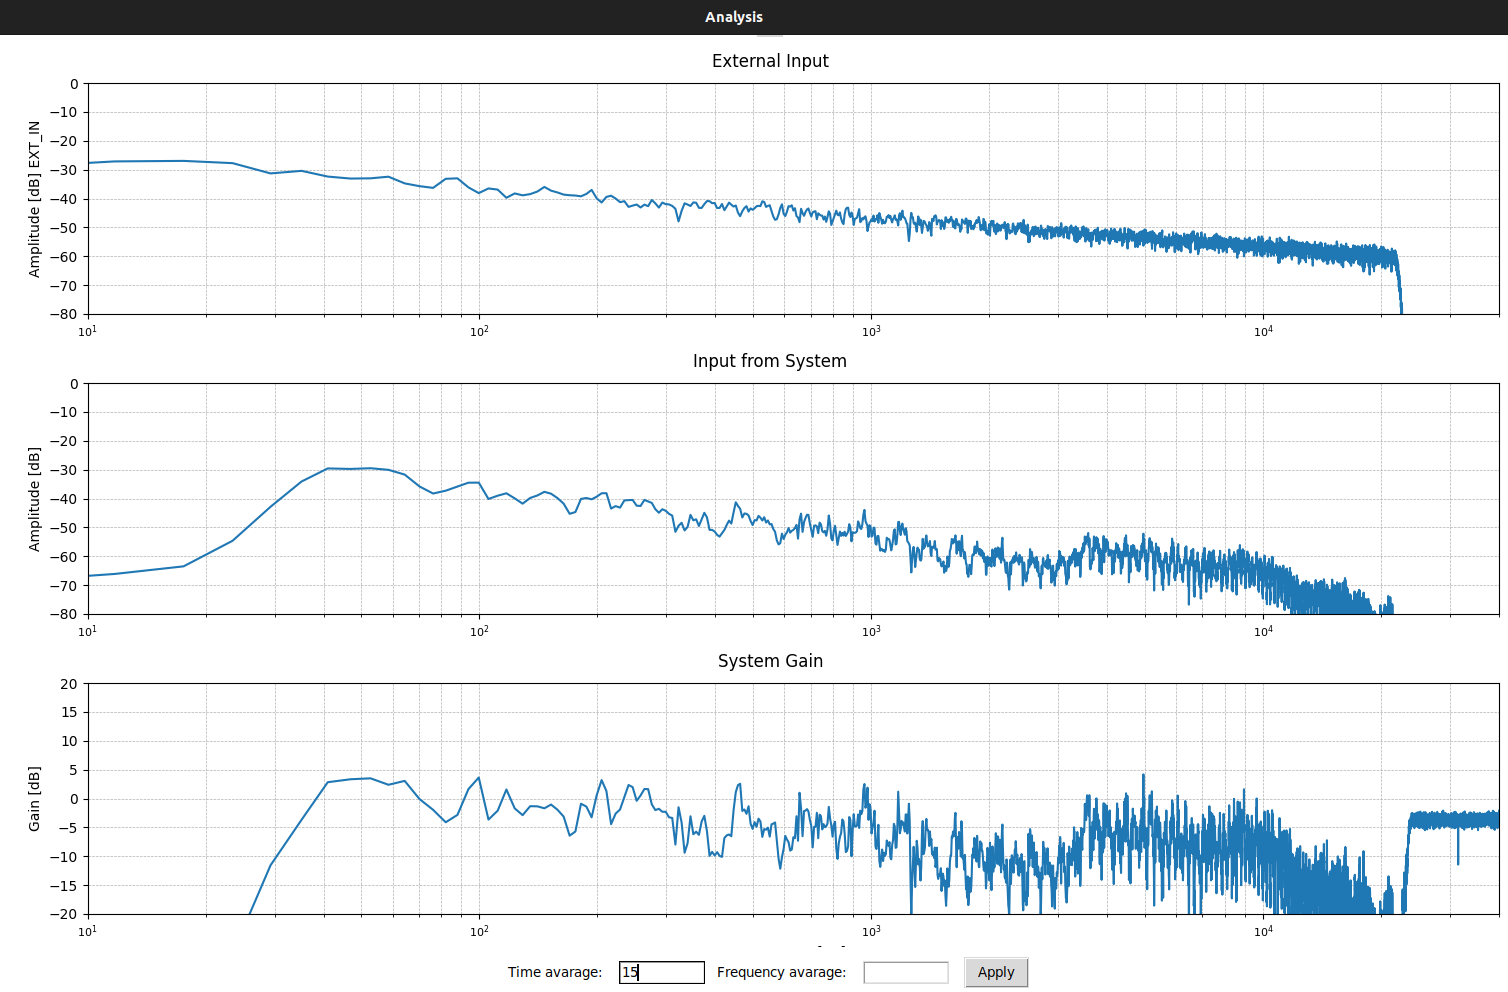
\includegraphics[width=0.6
	\linewidth]{Figures/Coro_FT_time_av.png}
	\caption{FT - Pink Noise - Time Avarage..............................................................}
	\label{fig:Coro_FT_time_av}
\end{figure}

\begin{figure}[H]
	\centering
	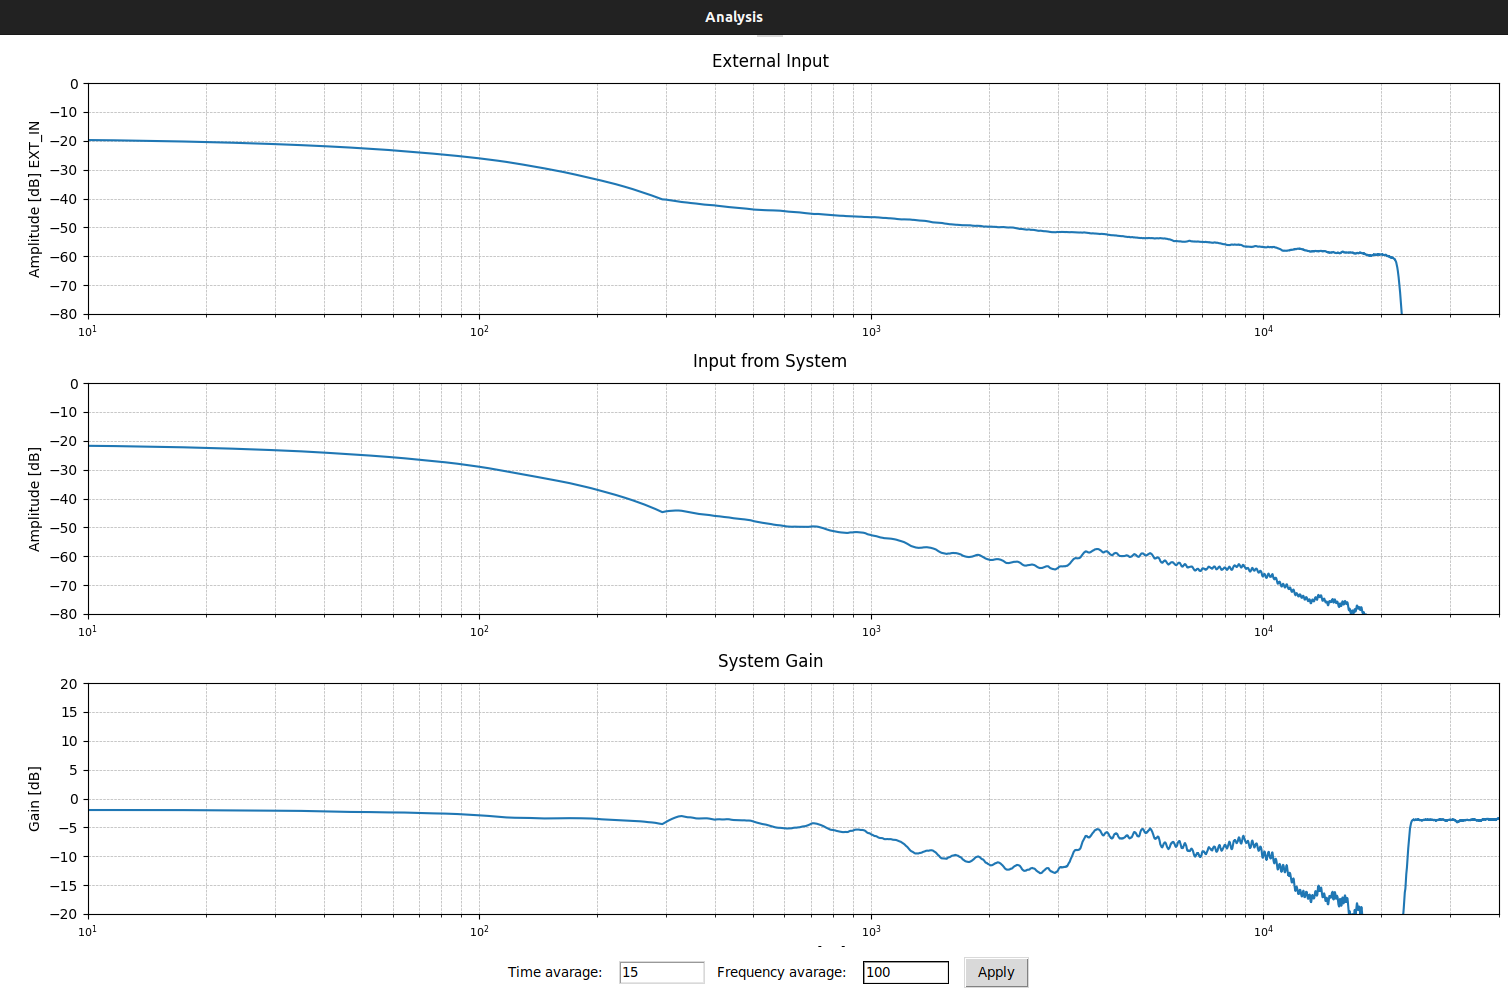
\includegraphics[width=0.6
	\linewidth]{Figures/Coro_FT_WITH_av.png}
	\caption{FT - Pink Noise - Time Avarage + Frequency Average...........................................}
	\label{fig:Coro_FT_av}
\end{figure}

\begin{figure}[H]
	\centering
	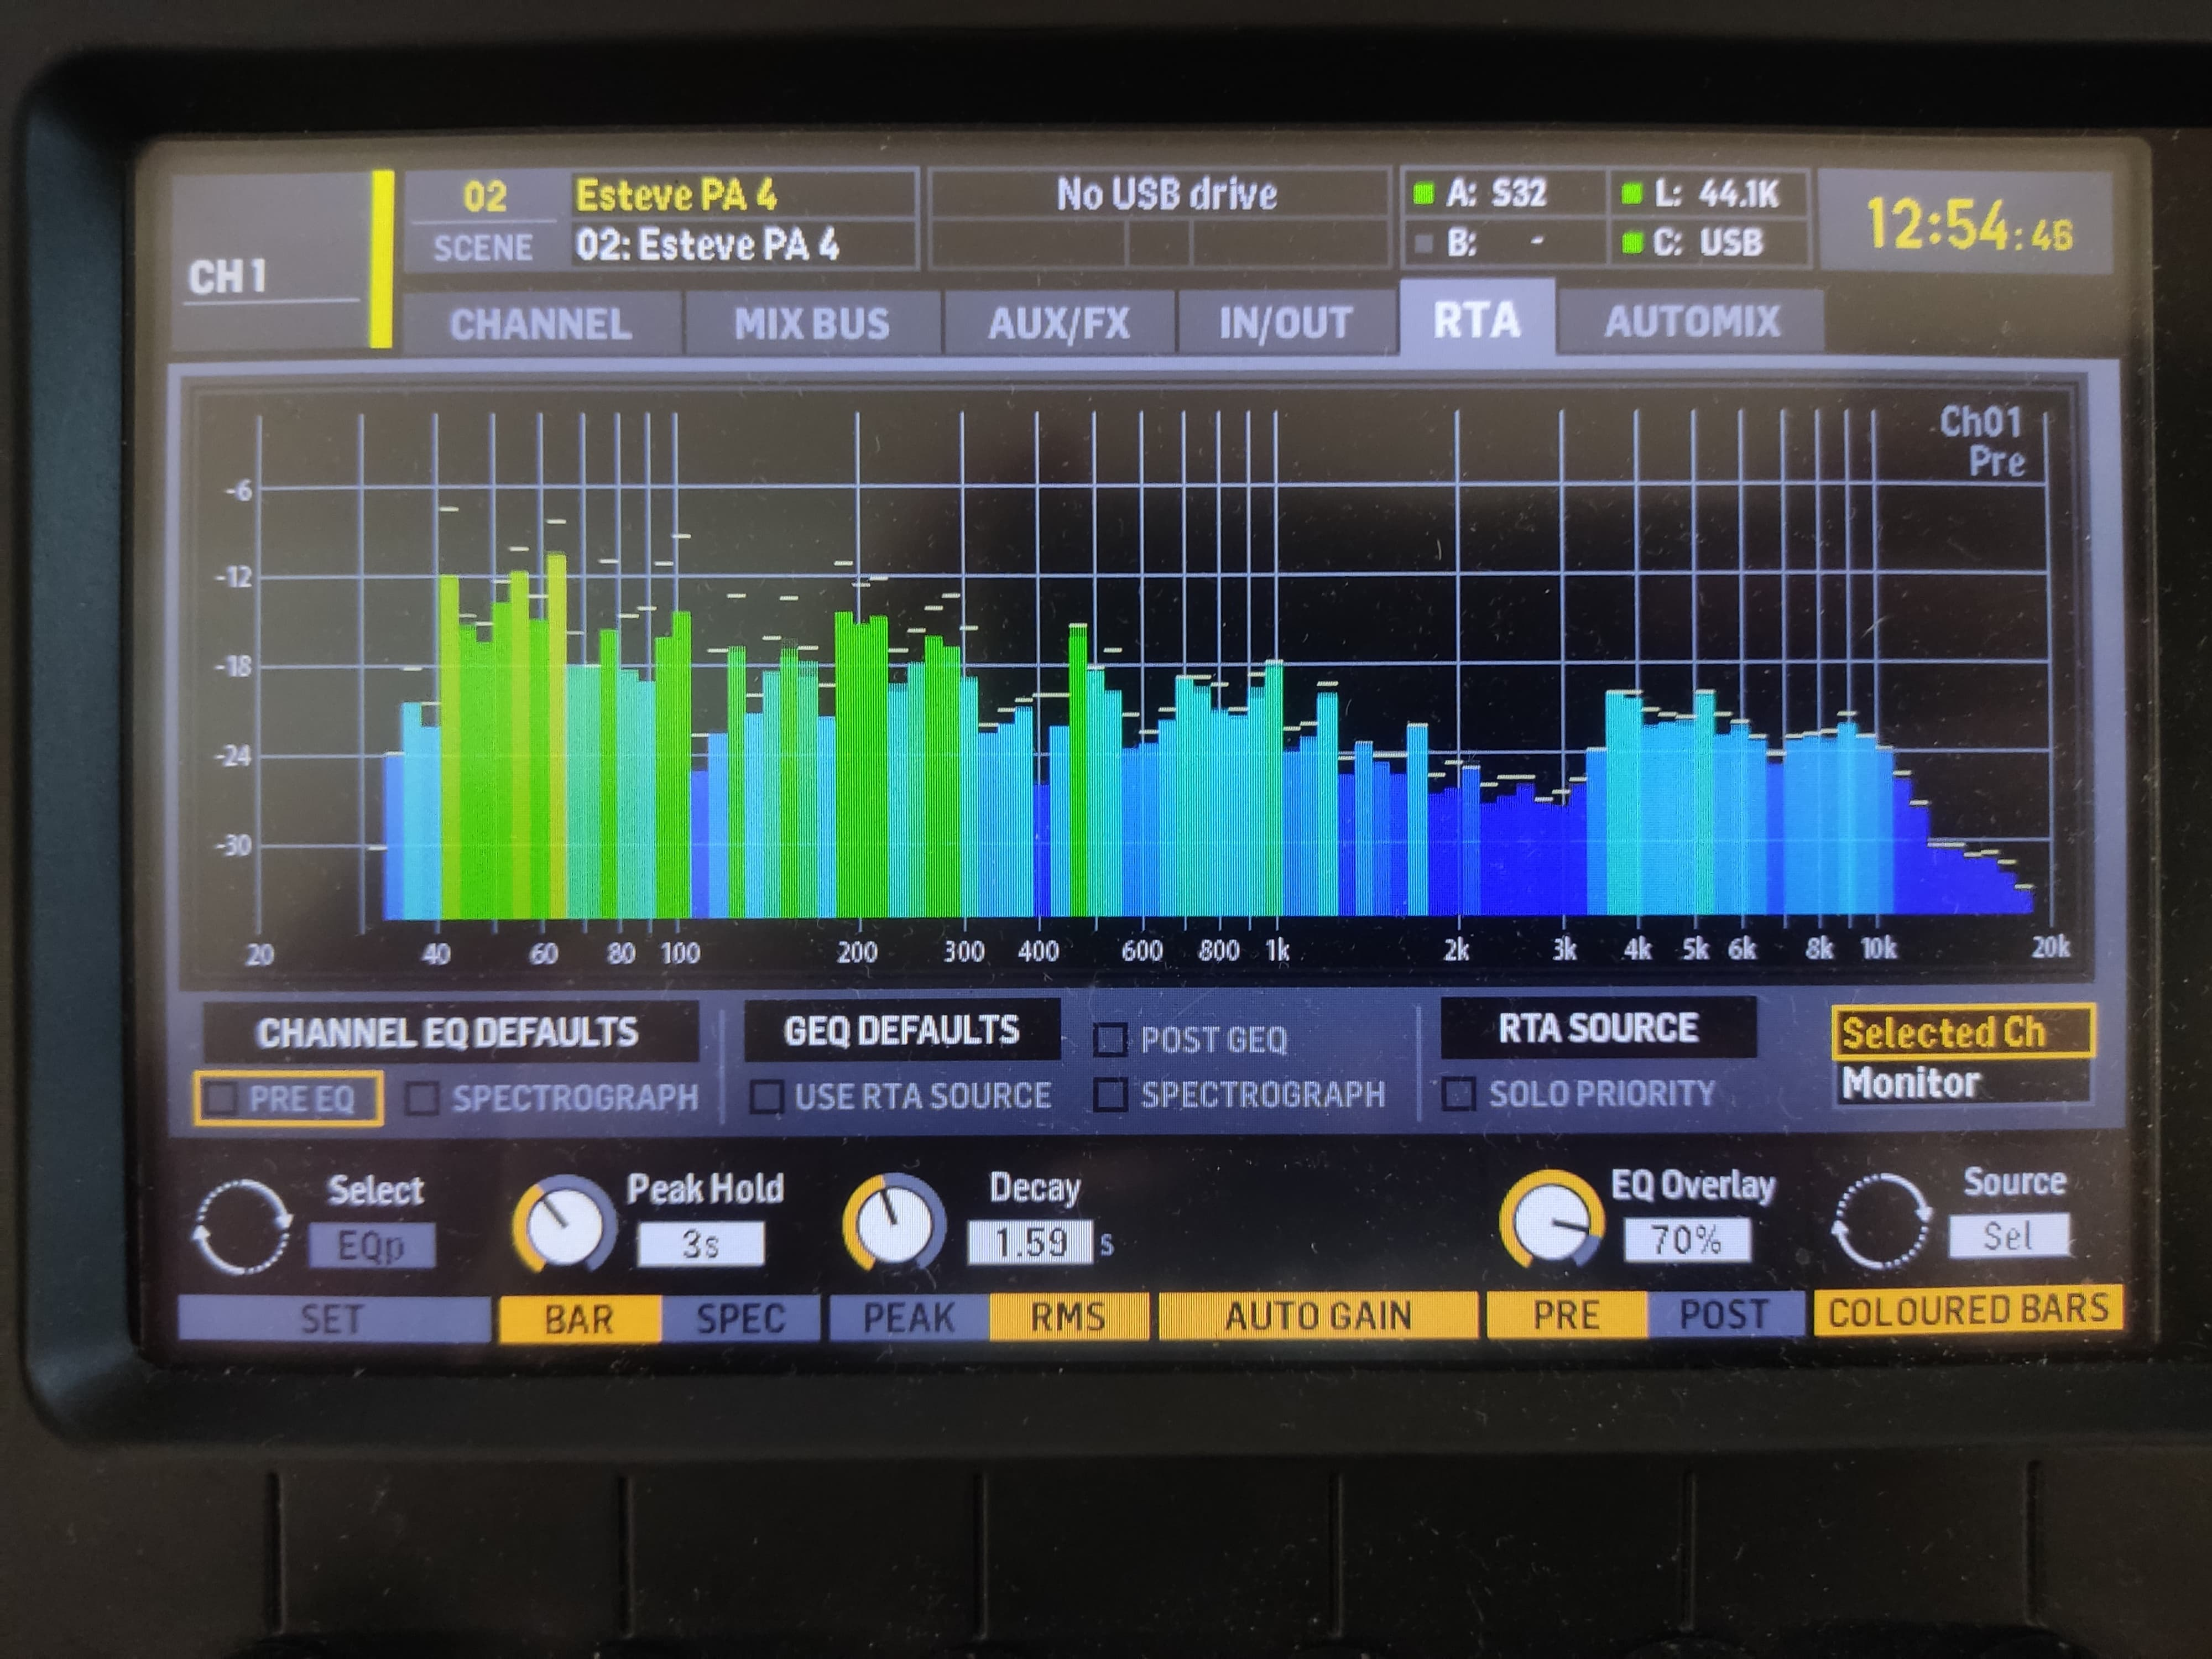
\includegraphics[width=0.6
	\linewidth]{Figures/Coro_X32_nontreated.jpeg}
	\caption{Microphone caption without any treatment, using X32 analysis tool....................}
	\label{fig:Coro_X32_nontreated}
\end{figure}

\begin{figure}[H]
	\centering
	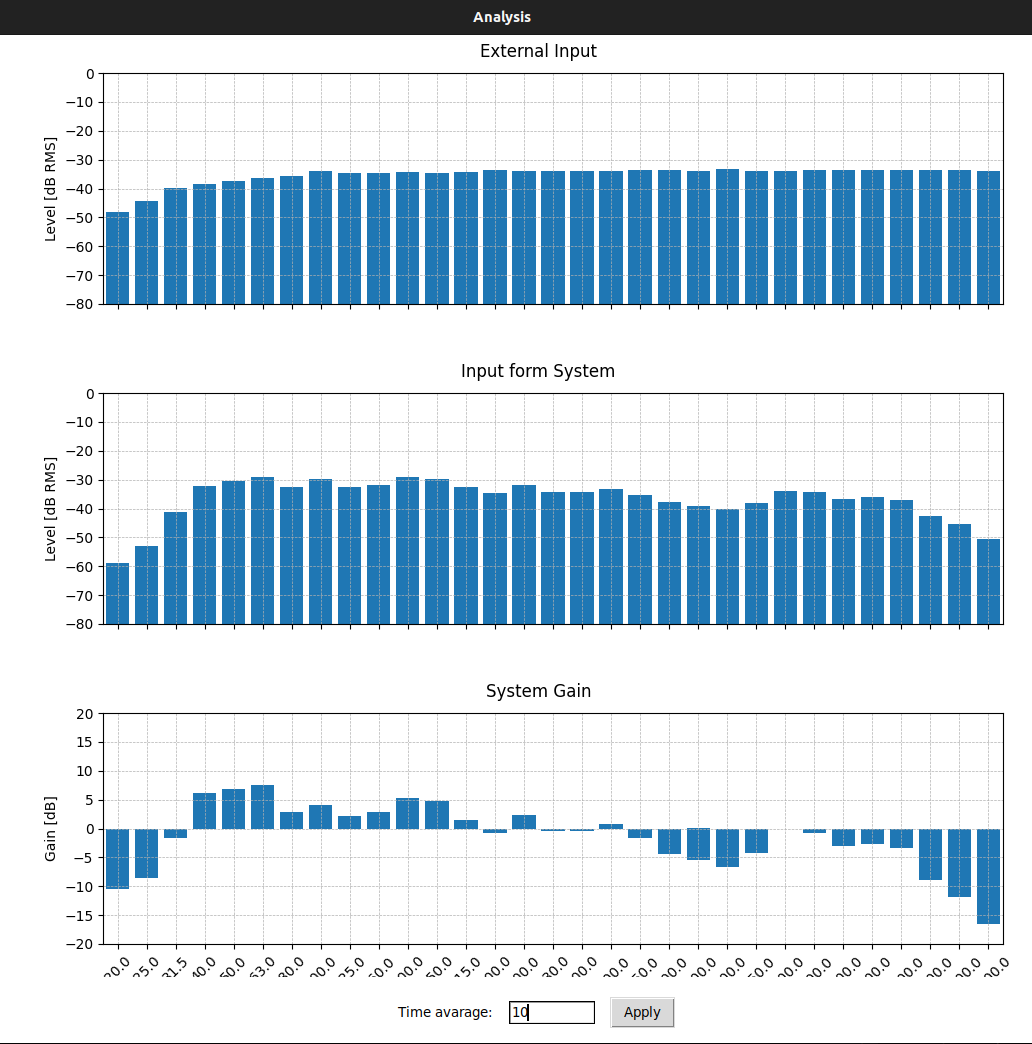
\includegraphics[width=0.6
	\linewidth]{Figures/Coro_RTA_Saved.png}
	\caption{Non treated Pink Noise, Saved results..............................................................}
	\label{fig:Coro_RTA_saved}
\end{figure}

\begin{figure}[H]
	\centering
	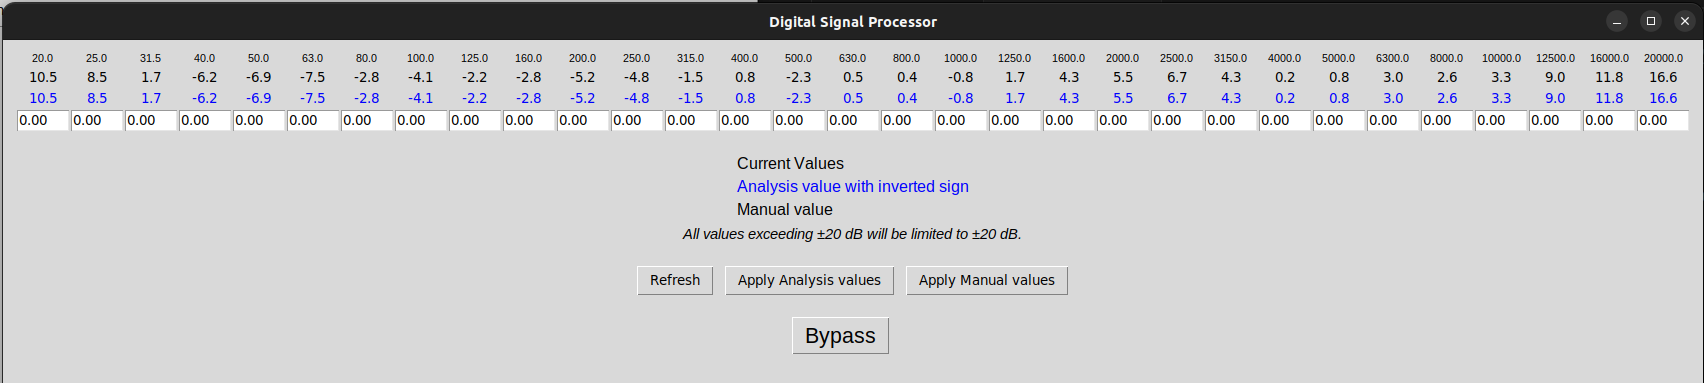
\includegraphics[width=1
	\linewidth]{Figures/Coro_EQ_from_RTA.png}
	\caption{EQ values applyed form RTA analysis..............................................................}
	\label{fig:Coro_EQ_RTA+C}
\end{figure}

\begin{figure}[H]
	\centering
	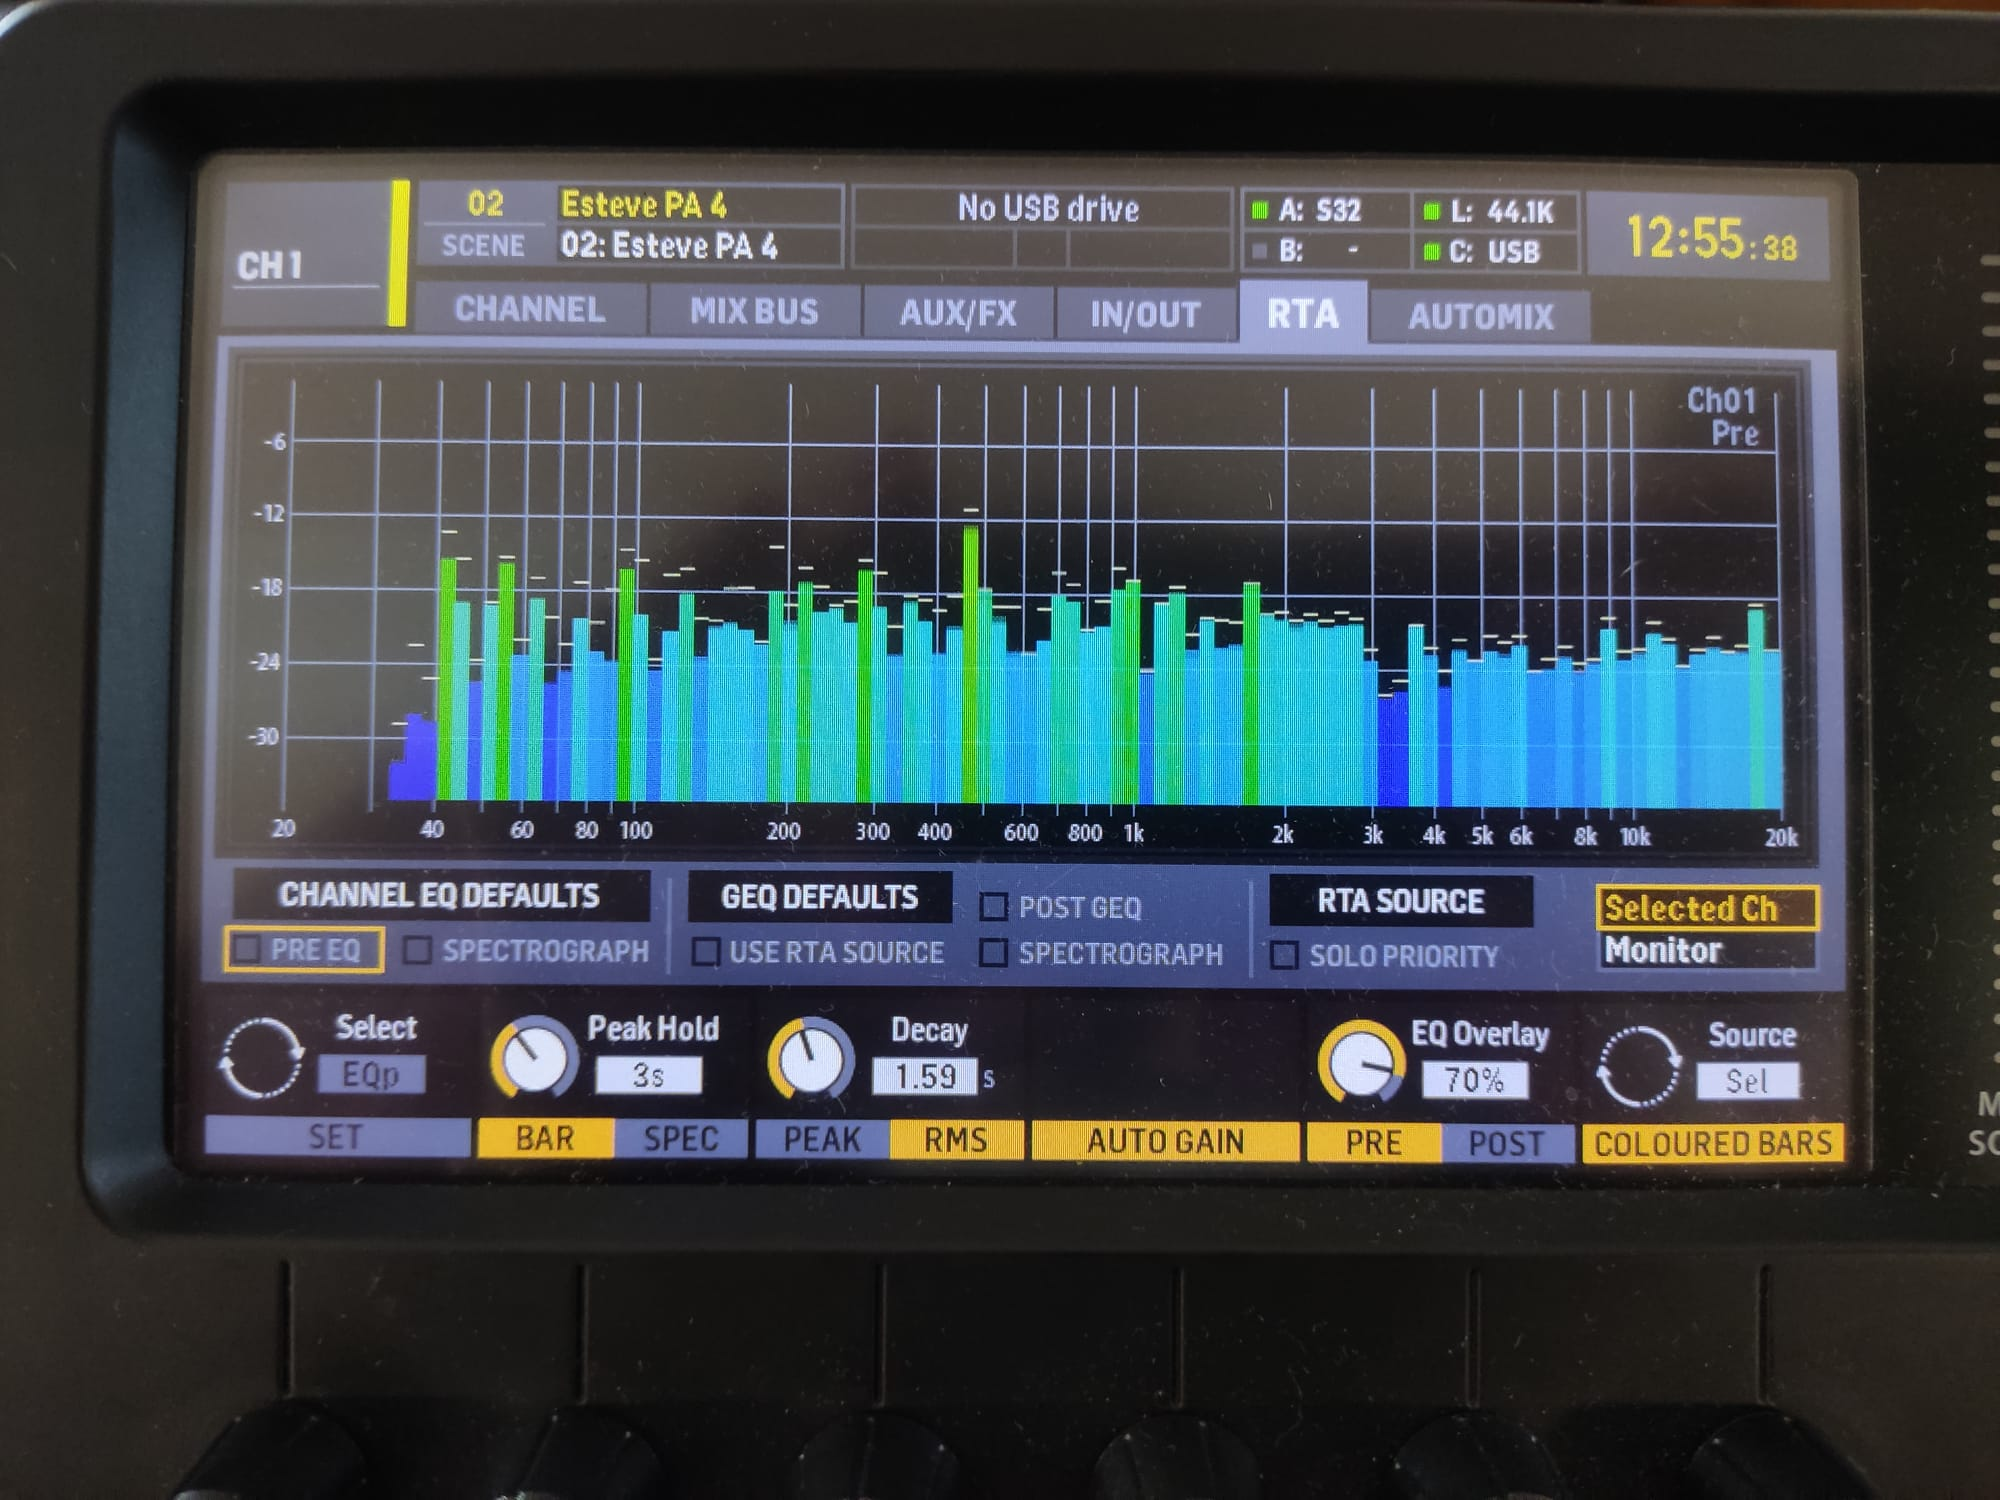
\includegraphics[width=0.6
	\linewidth]{Figures/Coro_X32_treatedRTAc.jpeg}
	\caption{Microphone caption with treatment by RTA+C, using X32 analysis tool..................}
	\label{fig:Coro_X32_RTA+C}
\end{figure}

\begin{figure}[H]
	\centering
	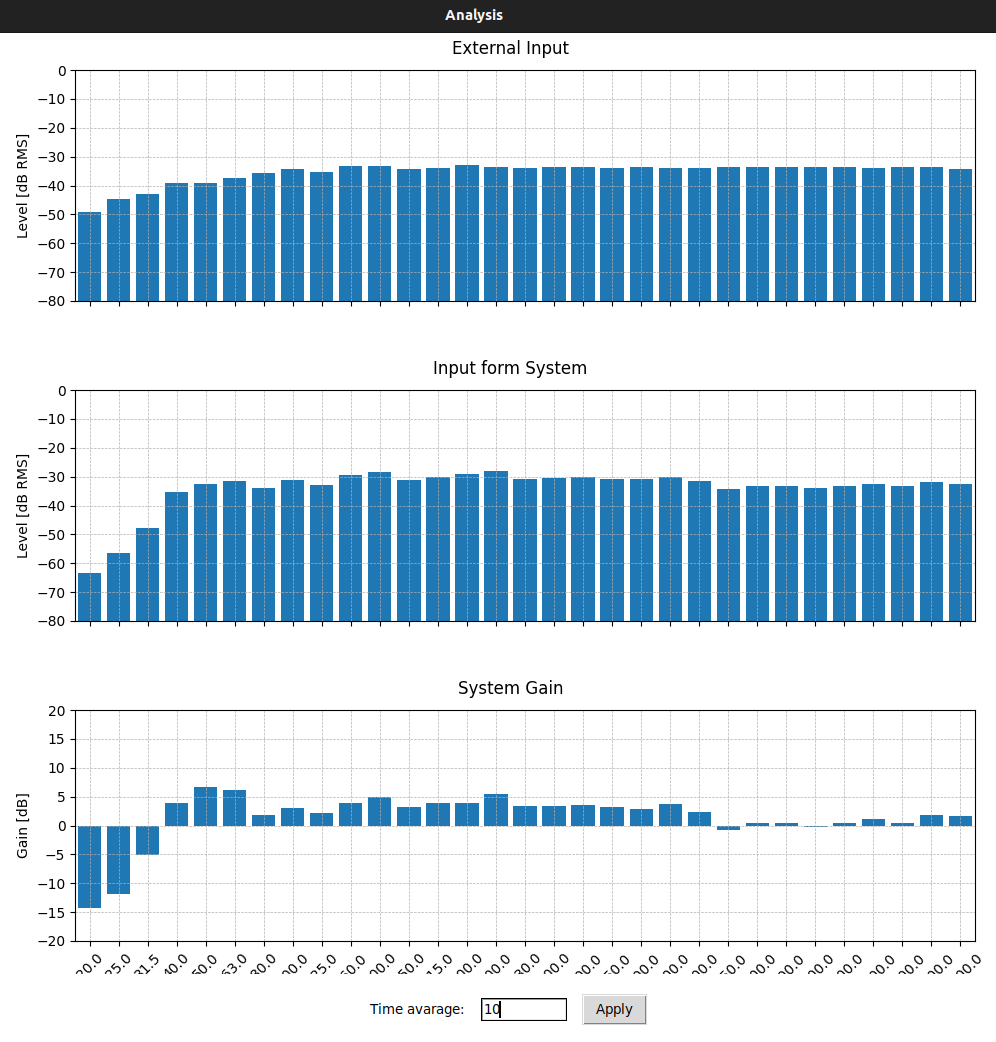
\includegraphics[width=0.6
	\linewidth]{Figures/Coro_RTA+EQ_ON.png}
	\caption{Pink Noise with processed signal by RTA+C program..............................................................}
	\label{fig:Coro_RTA_RTA+C}
\end{figure}

\begin{figure}[H]
	\centering
	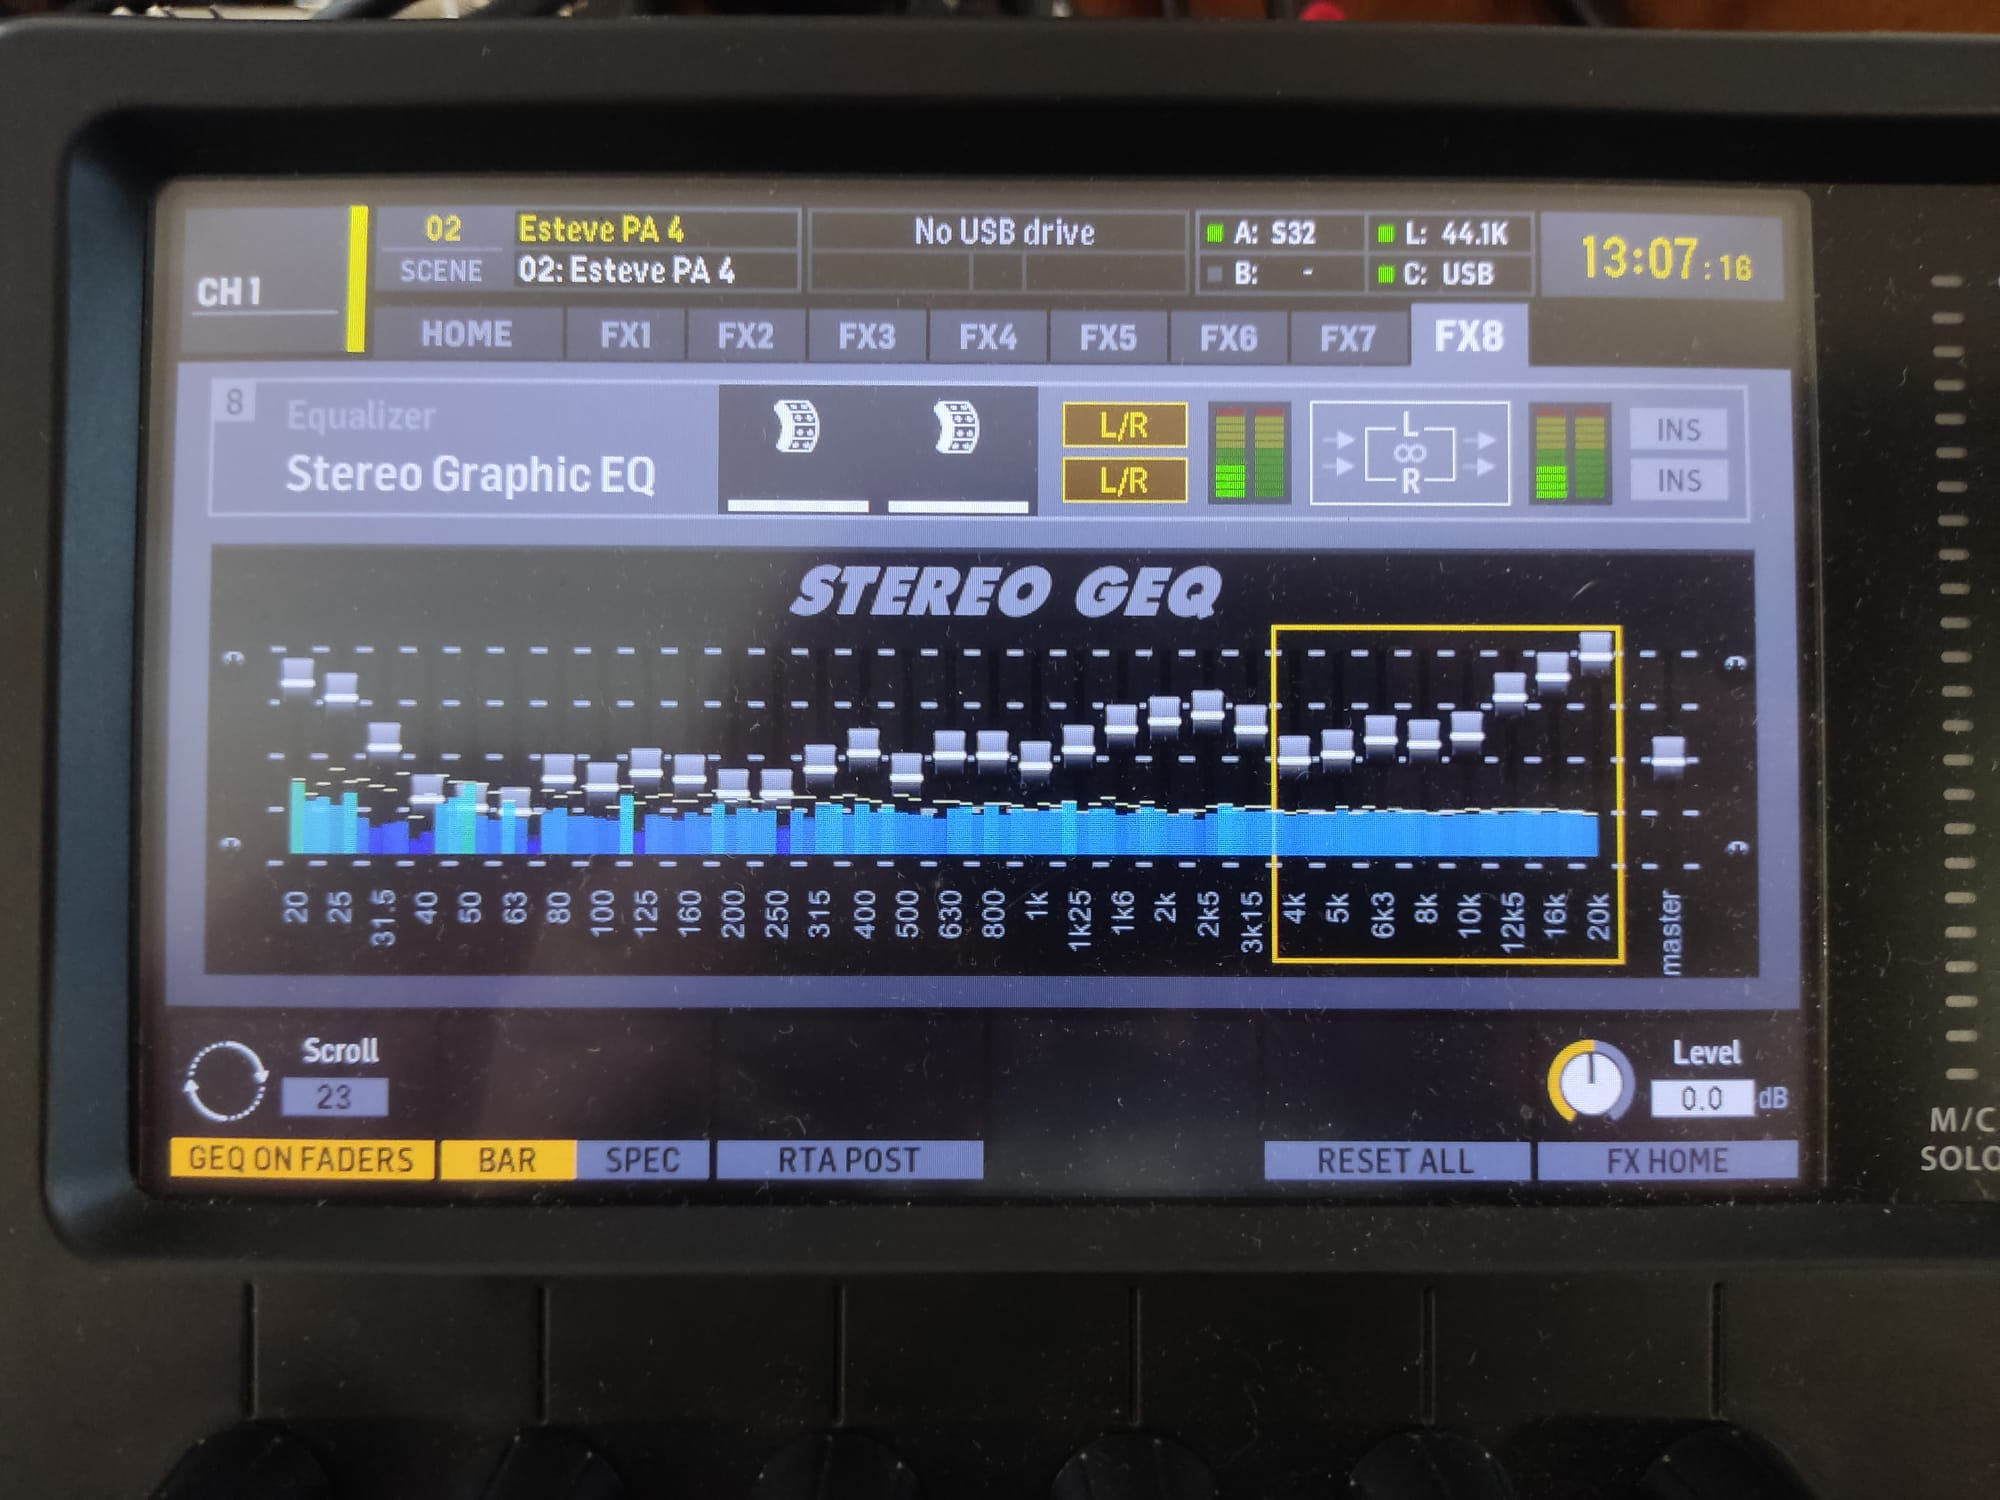
\includegraphics[width=0.6
	\linewidth]{Figures/Coro_X32_EQ.jpeg}
	\caption{Setting X32 EQ tool with parameters of RTA+C ........................................}
	\label{fig:Coro_X32_EQ}
\end{figure}

\begin{figure}[H]
	\centering
	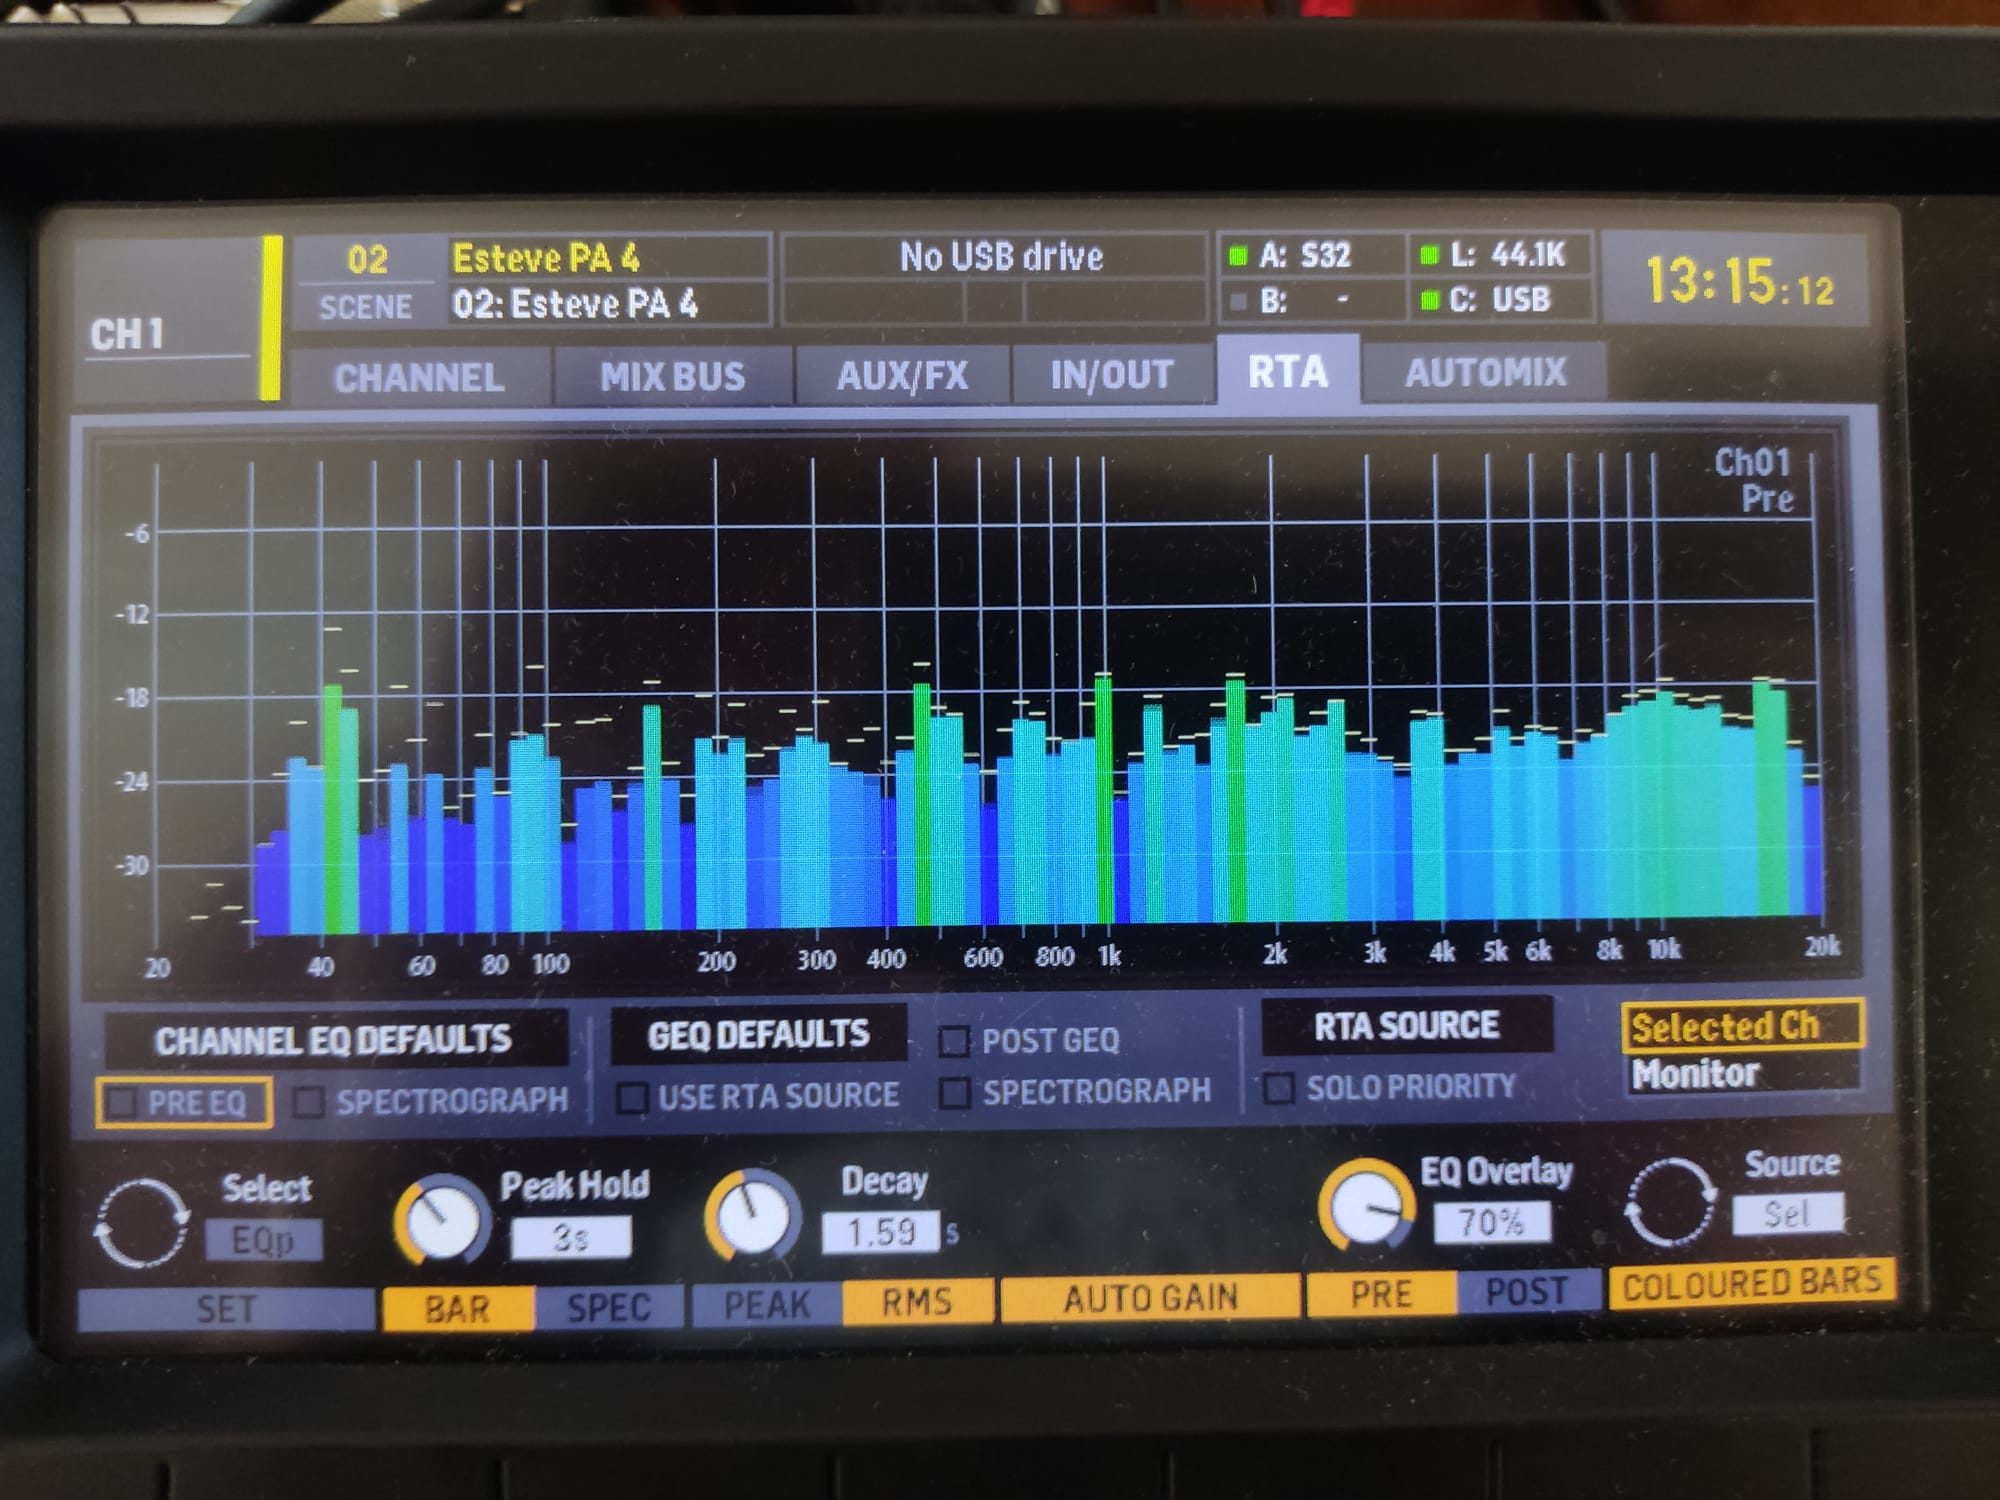
\includegraphics[width=0.6
	\linewidth]{Figures/Coro_X32_treatedX32.jpeg}
	\caption{Microphone caption with treatment of X32-EQ tool and using X32 analysis tool.........}
	\label{fig:Coro_X32_treatedX32}
\end{figure}

For music, use X32 EQ becouse the glitch ....................................................................

\begin{figure}[H]
	\centering
	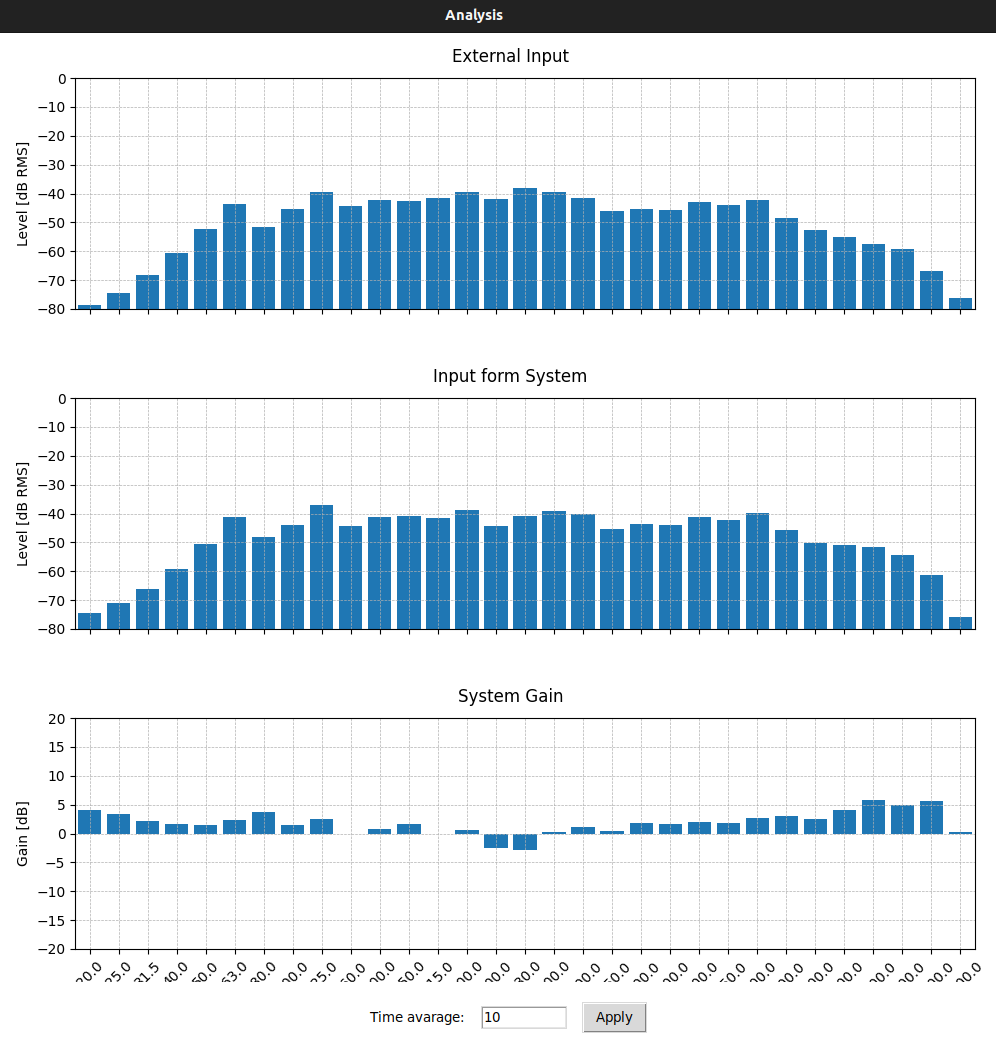
\includegraphics[width=0.6
	\linewidth]{Figures/Coro_Music_EQ_X32.png}
	\caption{RTA, using music, and EQ from X32..............................................................}
	\label{fig:Coro_RTA_music}
\end{figure}

\begin{figure}[H]
	\centering
	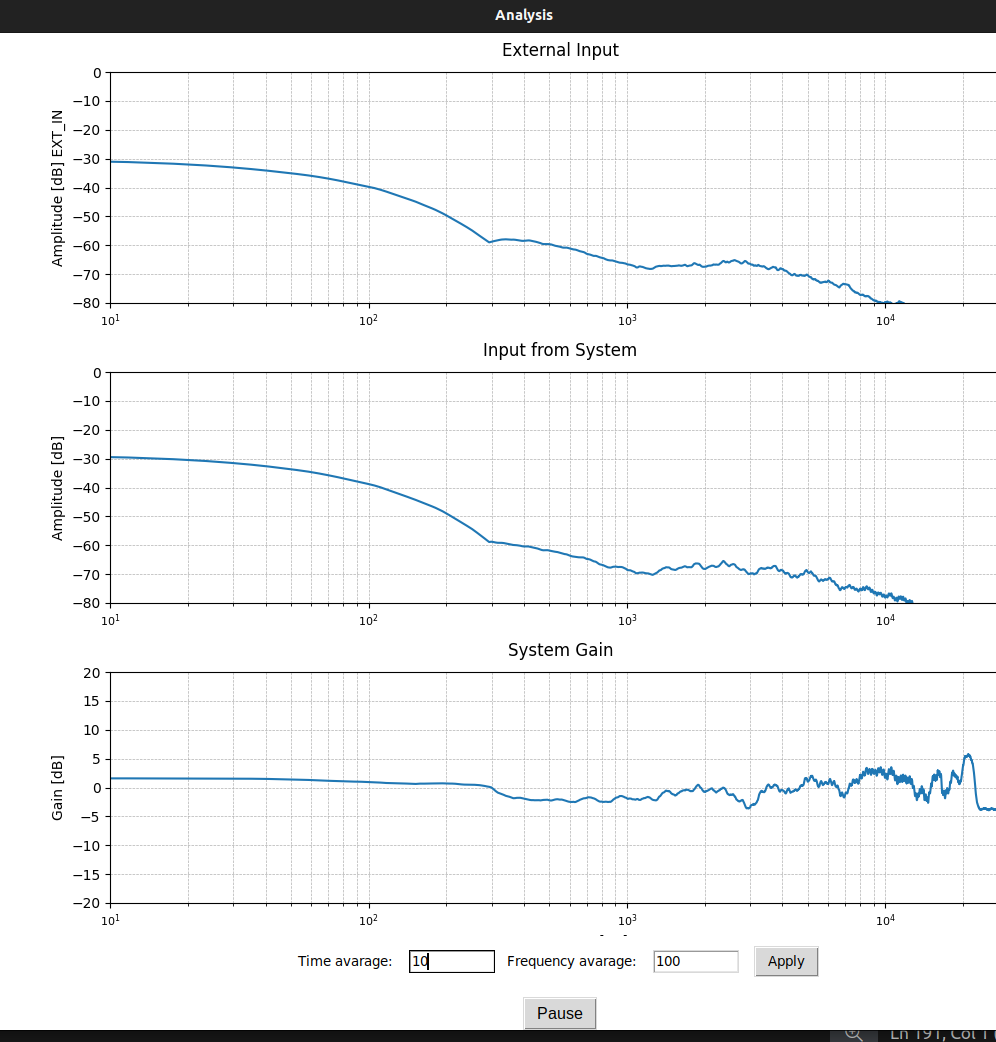
\includegraphics[width=0.6
	\linewidth]{Figures/Coro_FT_music_EQX32.png}
	\caption{FT, using music, and EQ from X32..............................................................}
	\label{fig:Coro_FT_music}
\end{figure}

Looks preaty nice .......................................................................


\section{User experiance}

About user experiance.

